\documentclass[11pt,a4paper]{article}

\usepackage[utf8]{inputenc}
\usepackage[T1]{fontenc}
\usepackage[provide=*,spanish]{babel}
\usepackage{amsmath}
\usepackage{amssymb}
\usepackage{booktabs}
\usepackage{graphicx}
\usepackage{subcaption}
\usepackage{geometry}
\usepackage[expansion=false]{microtype}
\usepackage[hidelinks]{hyperref}

\geometry{
    top=2.5cm,
    bottom=2.5cm,
    left=2.5cm,
    right=2.5cm
}

\title{Validación del paso temporal y elección de la regularización}
\author{}
\date{}

\begin{document}

\maketitle

\section{Objetivo}

Luego de introducir la regularización del núcleo de la interacción, quedan dos
elecciones que deben cerrarse antes de continuar con el protocolo numérico:
el valor de \(\lambda\), que controla cuánto se refuerza la repulsión a
superposiciones altas, y el paso temporal de integración \(\Delta t\).

El objetivo de este análisis es verificar que los observables relevantes sean
estables al reducir \(\Delta t\), estudiar si aparecen superposiciones o
velocidades anómalas y, con esos resultados, seleccionar valores de producción
que sean físicamente razonables y computacionalmente manejables.

\section{Protocolo}

Se realizaron simulaciones con

\begin{equation}
\lambda\in\{0.1,1\},
\qquad
\Delta t\in
\{0.001,0.002,0.005,0.01,0.025,0.05,0.1\},
\end{equation}

usando \(N=1000\), \(k=2.5\), \(\gamma=3\), sin ruido, condición inicial
aleatoria con todas las células redondas y deformación instantánea.

Para cada combinación se simularon 64 realizaciones para

\begin{equation}
\rho\in\{0.75,0.80,0.84,0.90\},
\end{equation}

hasta \(t=2000\). Los promedios tardíos se calcularon en la ventana

\begin{equation}
1500\leq t\leq2000.
\end{equation}

Las mismas semillas se reutilizaron en toda la campaña. Sin embargo, para
evaluar convergencia a tiempos largos no exigimos que dos trayectorias con la
misma semilla permanezcan cercanas punto a punto: pequeñas diferencias
numéricas pueden decorrelacionar trayectorias individuales en una dinámica
colectiva no lineal. Por eso el criterio principal se basa en estadísticas de
ensamble.

\section{Ventana temporal tardía}

Antes de comparar los distintos pasos temporales, verificamos la evolución de
la fracción de células elongadas para la simulación mejor resuelta,
\(\Delta t=0.001\). La figura~\ref{fig:late_time} muestra que la ventana
\(1500\leq t\leq2000\) representa adecuadamente el régimen tardío de las
densidades estudiadas. En \(\rho=0.90\) puede persistir una evolución lenta,
por lo que hablamos de régimen tardío o cuasiestacionario y no necesariamente
de un estado estacionario estricto.

\begin{figure}[htbp]
    \centering
    \begin{subfigure}[t]{0.48\textwidth}
        \centering
        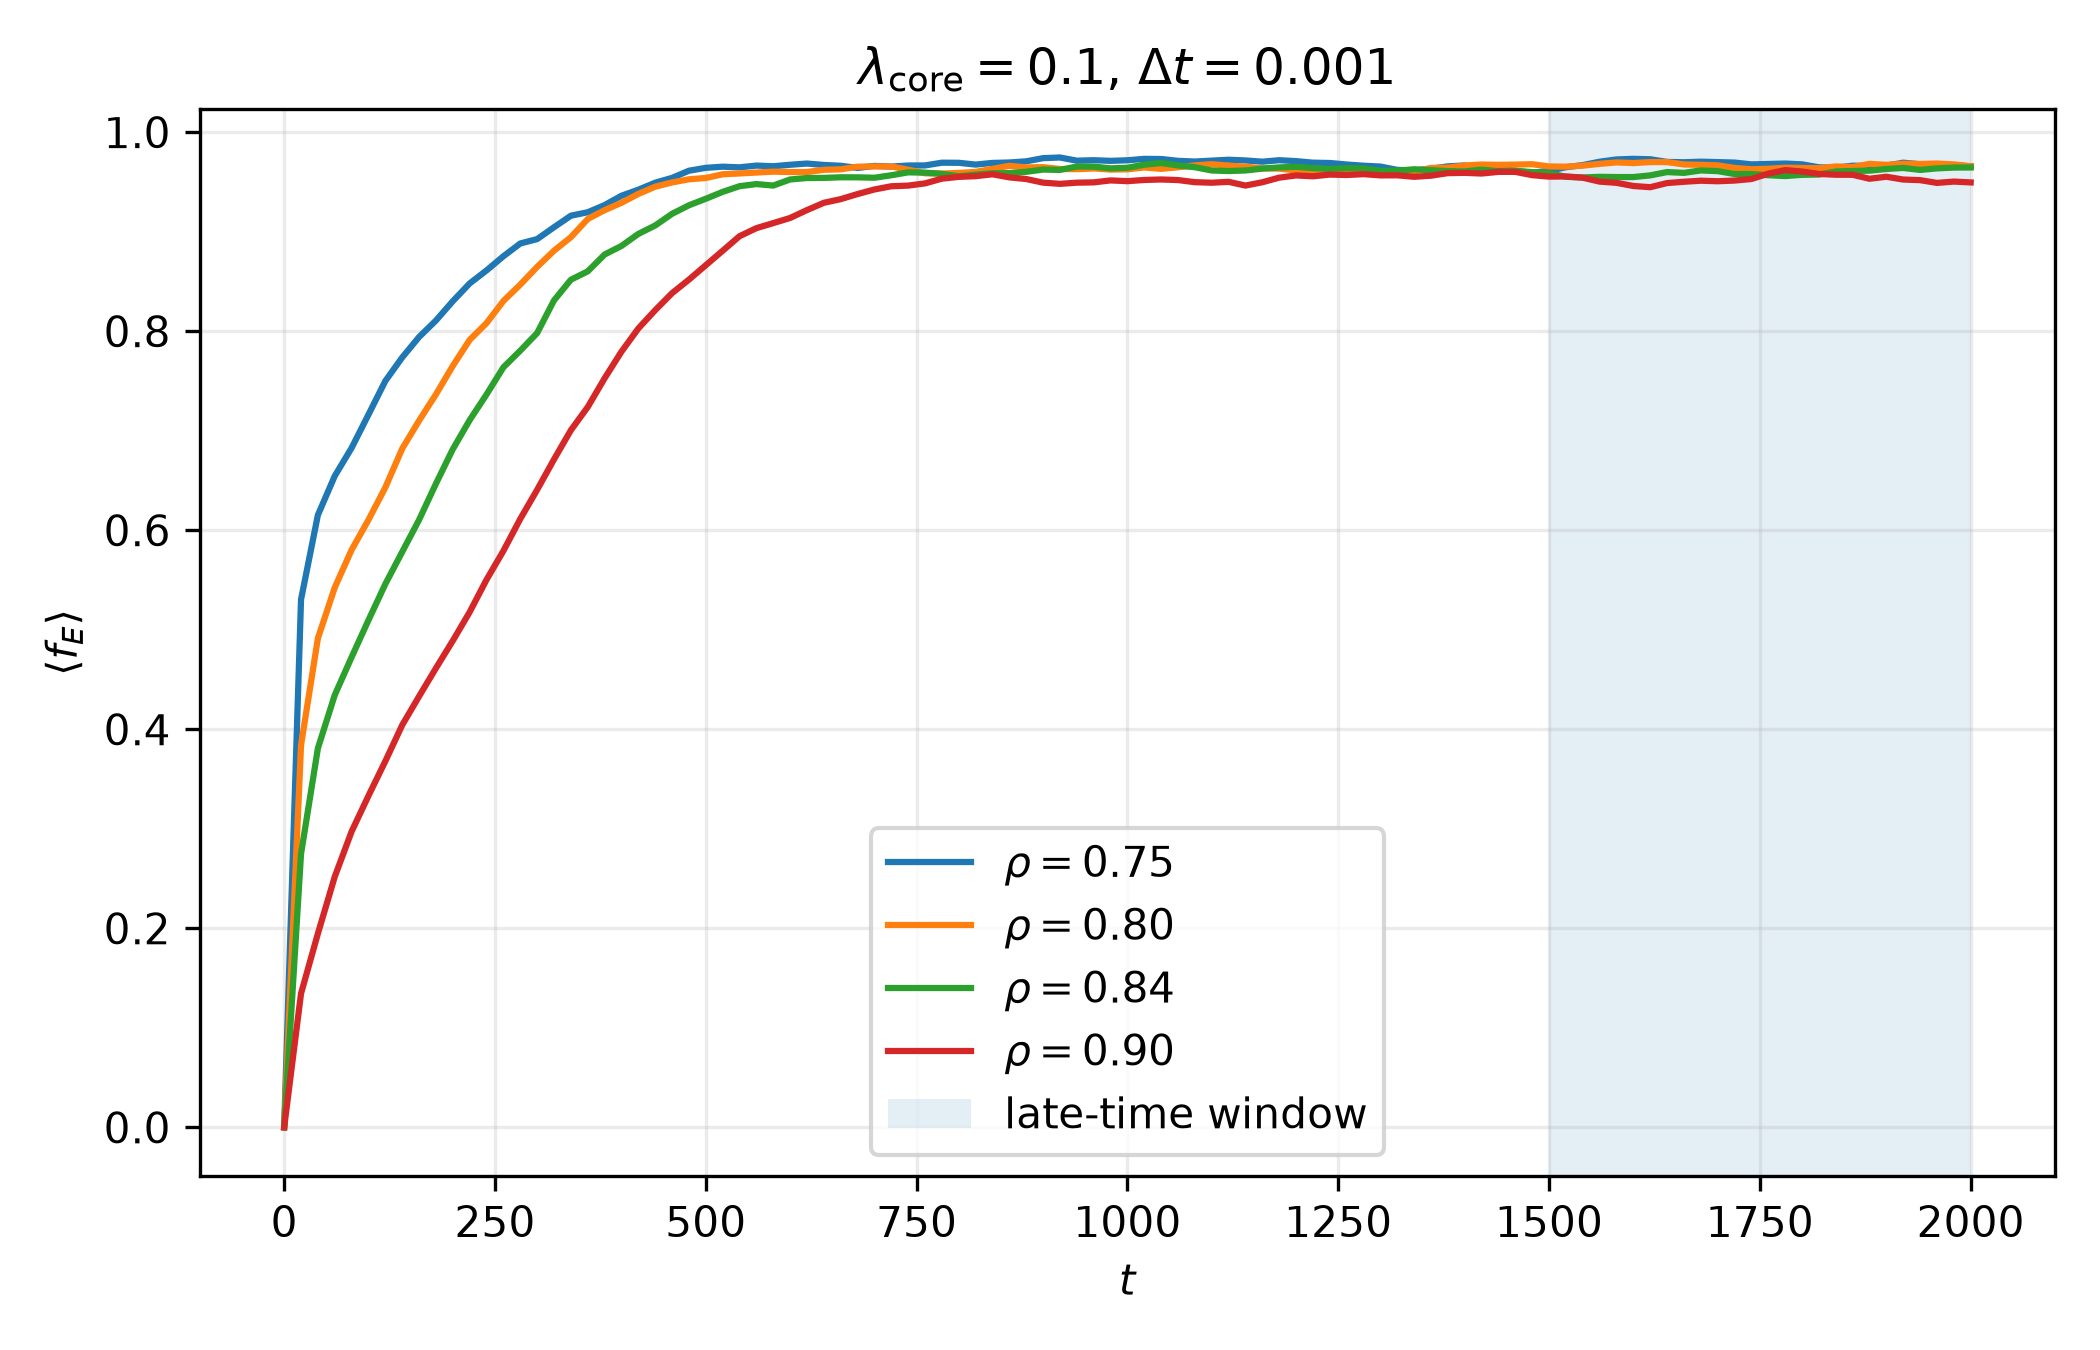
\includegraphics[width=\textwidth]
        {../figures/late_time_window_lambda_0.1.png}
        \caption{\(\lambda=0.1\).}
    \end{subfigure}
    \hfill
    \begin{subfigure}[t]{0.48\textwidth}
        \centering
        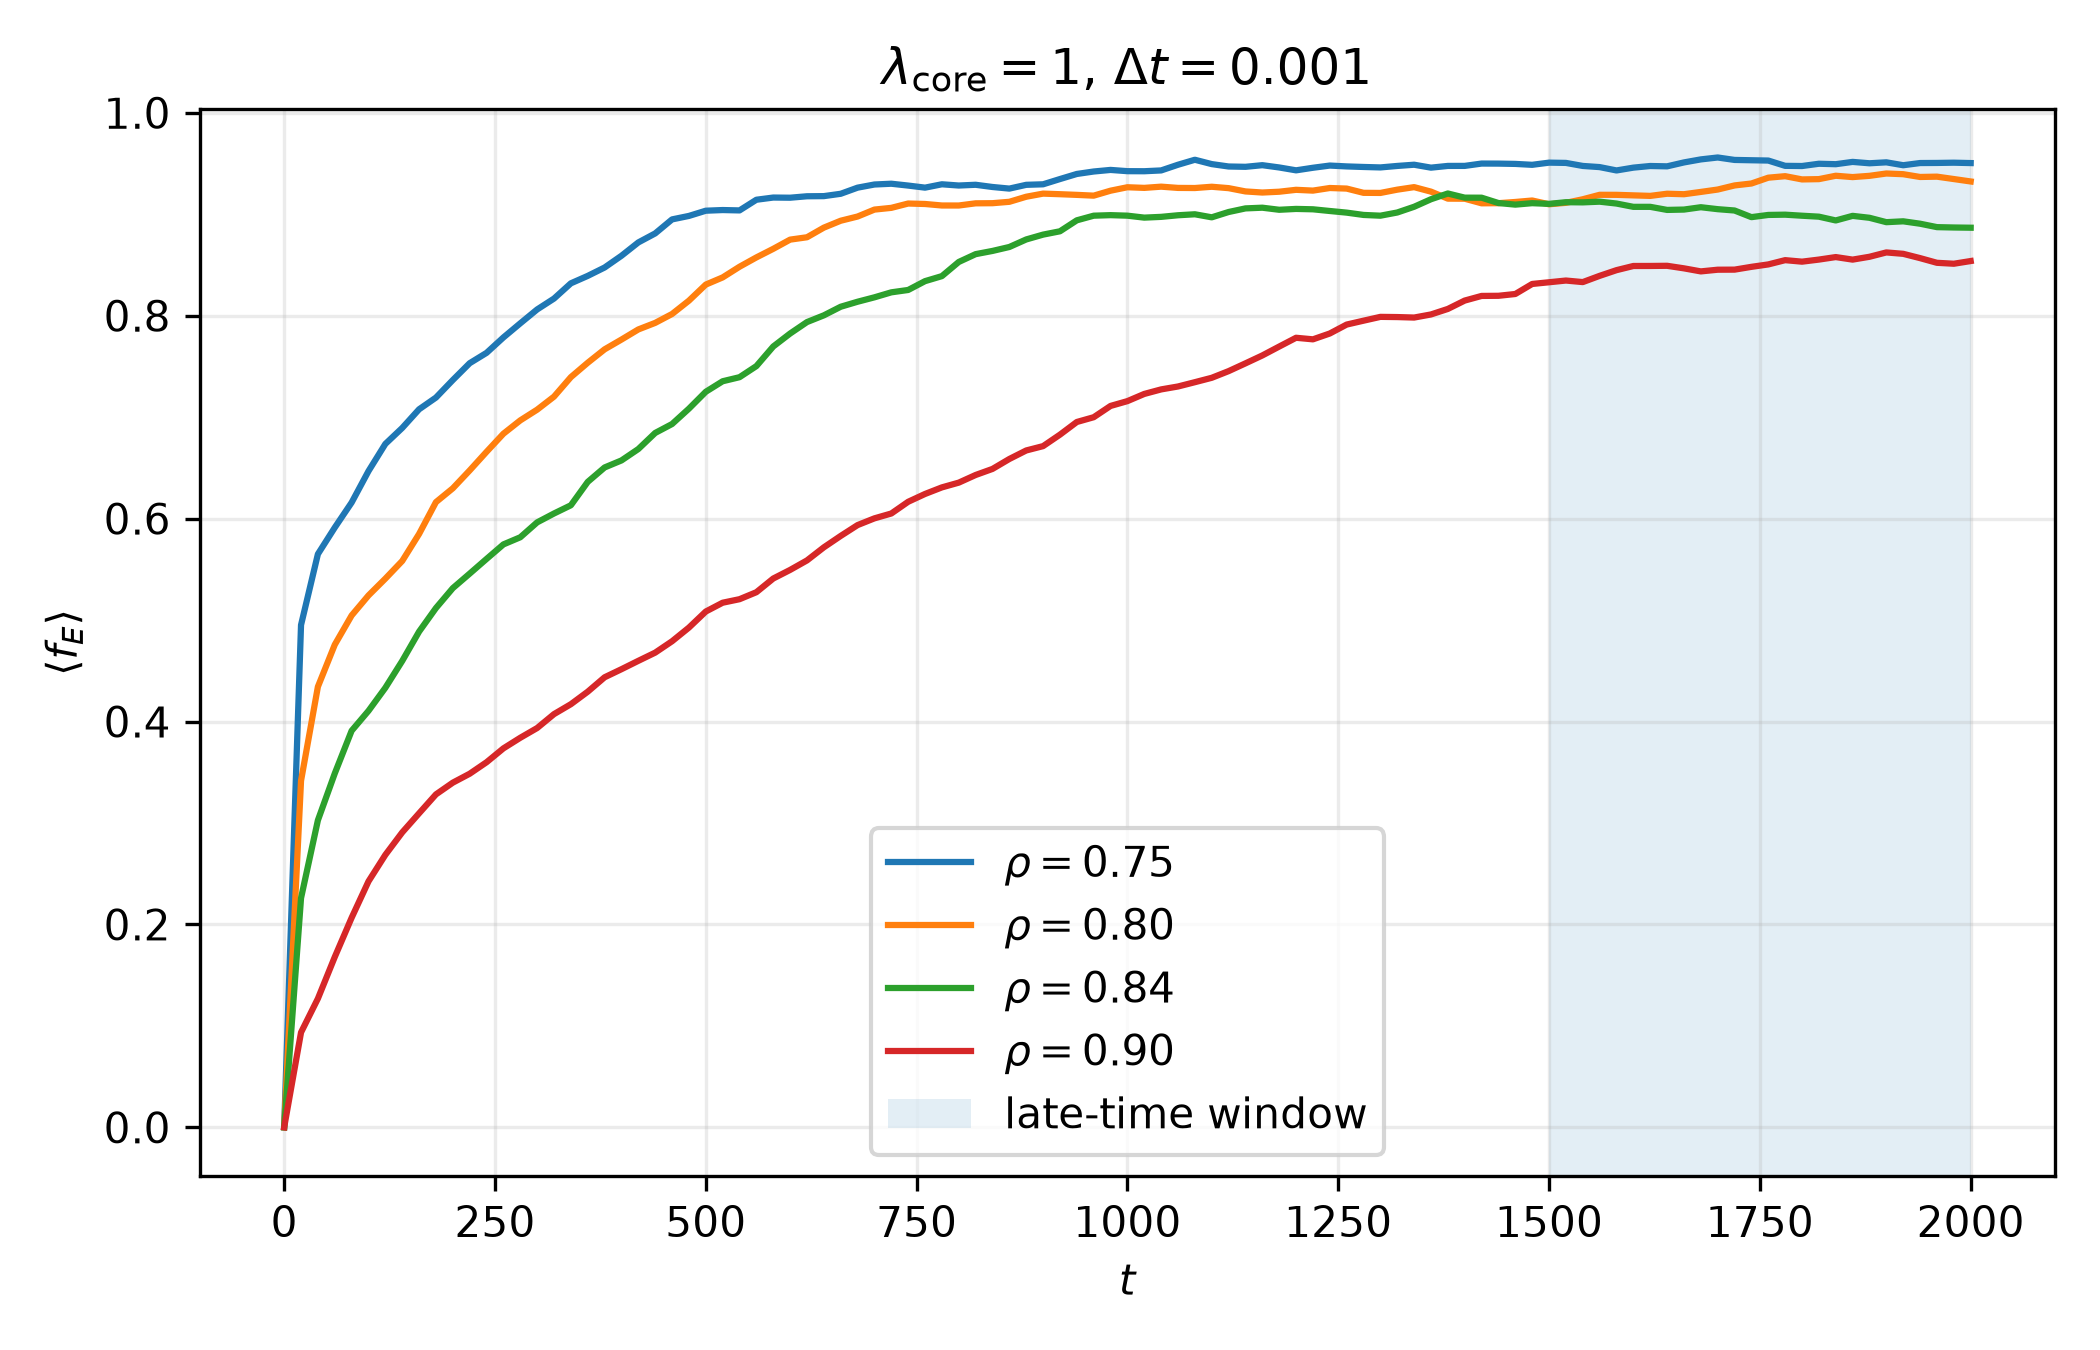
\includegraphics[width=\textwidth]
        {../figures/late_time_window_lambda_1.png}
        \caption{\(\lambda=1\).}
    \end{subfigure}
    \caption{
        Evolución temporal de la fracción de células elongadas para
        \(\Delta t=0.001\). La región sombreada corresponde a la ventana
        \(1500\leq t\leq2000\) utilizada para los promedios tardíos.
    }
    \label{fig:late_time}
\end{figure}

\section{Convergencia de los observables macroscópicos}

Consideramos cuatro cantidades que resumen el estado colectivo:

\begin{itemize}
    \item fracción de células elongadas \(f_E\);
    \item orden polar \(P\);
    \item orden nemático \(Q\);
    \item fracción \(S_{1,E}/N_E\) de células elongadas pertenecientes al
    mayor cluster espacial elongado.
\end{itemize}

La figura~\ref{fig:macro_stats} muestra las medias de ensamble y sus errores
estándar. Para \(\lambda=1\), los valores obtenidos para
\(\Delta t=0.001,0.002,0.005\) y \(0.01\) forman un mismo régimen estadístico.
En \(\Delta t=0.025\) comienzan a observarse cambios sistemáticos,
principalmente en la fracción elongada y en la estructura de clusters, y para
\(\Delta t\geq0.05\) las diferencias son claras.

\begin{figure}[htbp]
    \centering
    \begin{subfigure}[t]{0.48\textwidth}
        \centering
        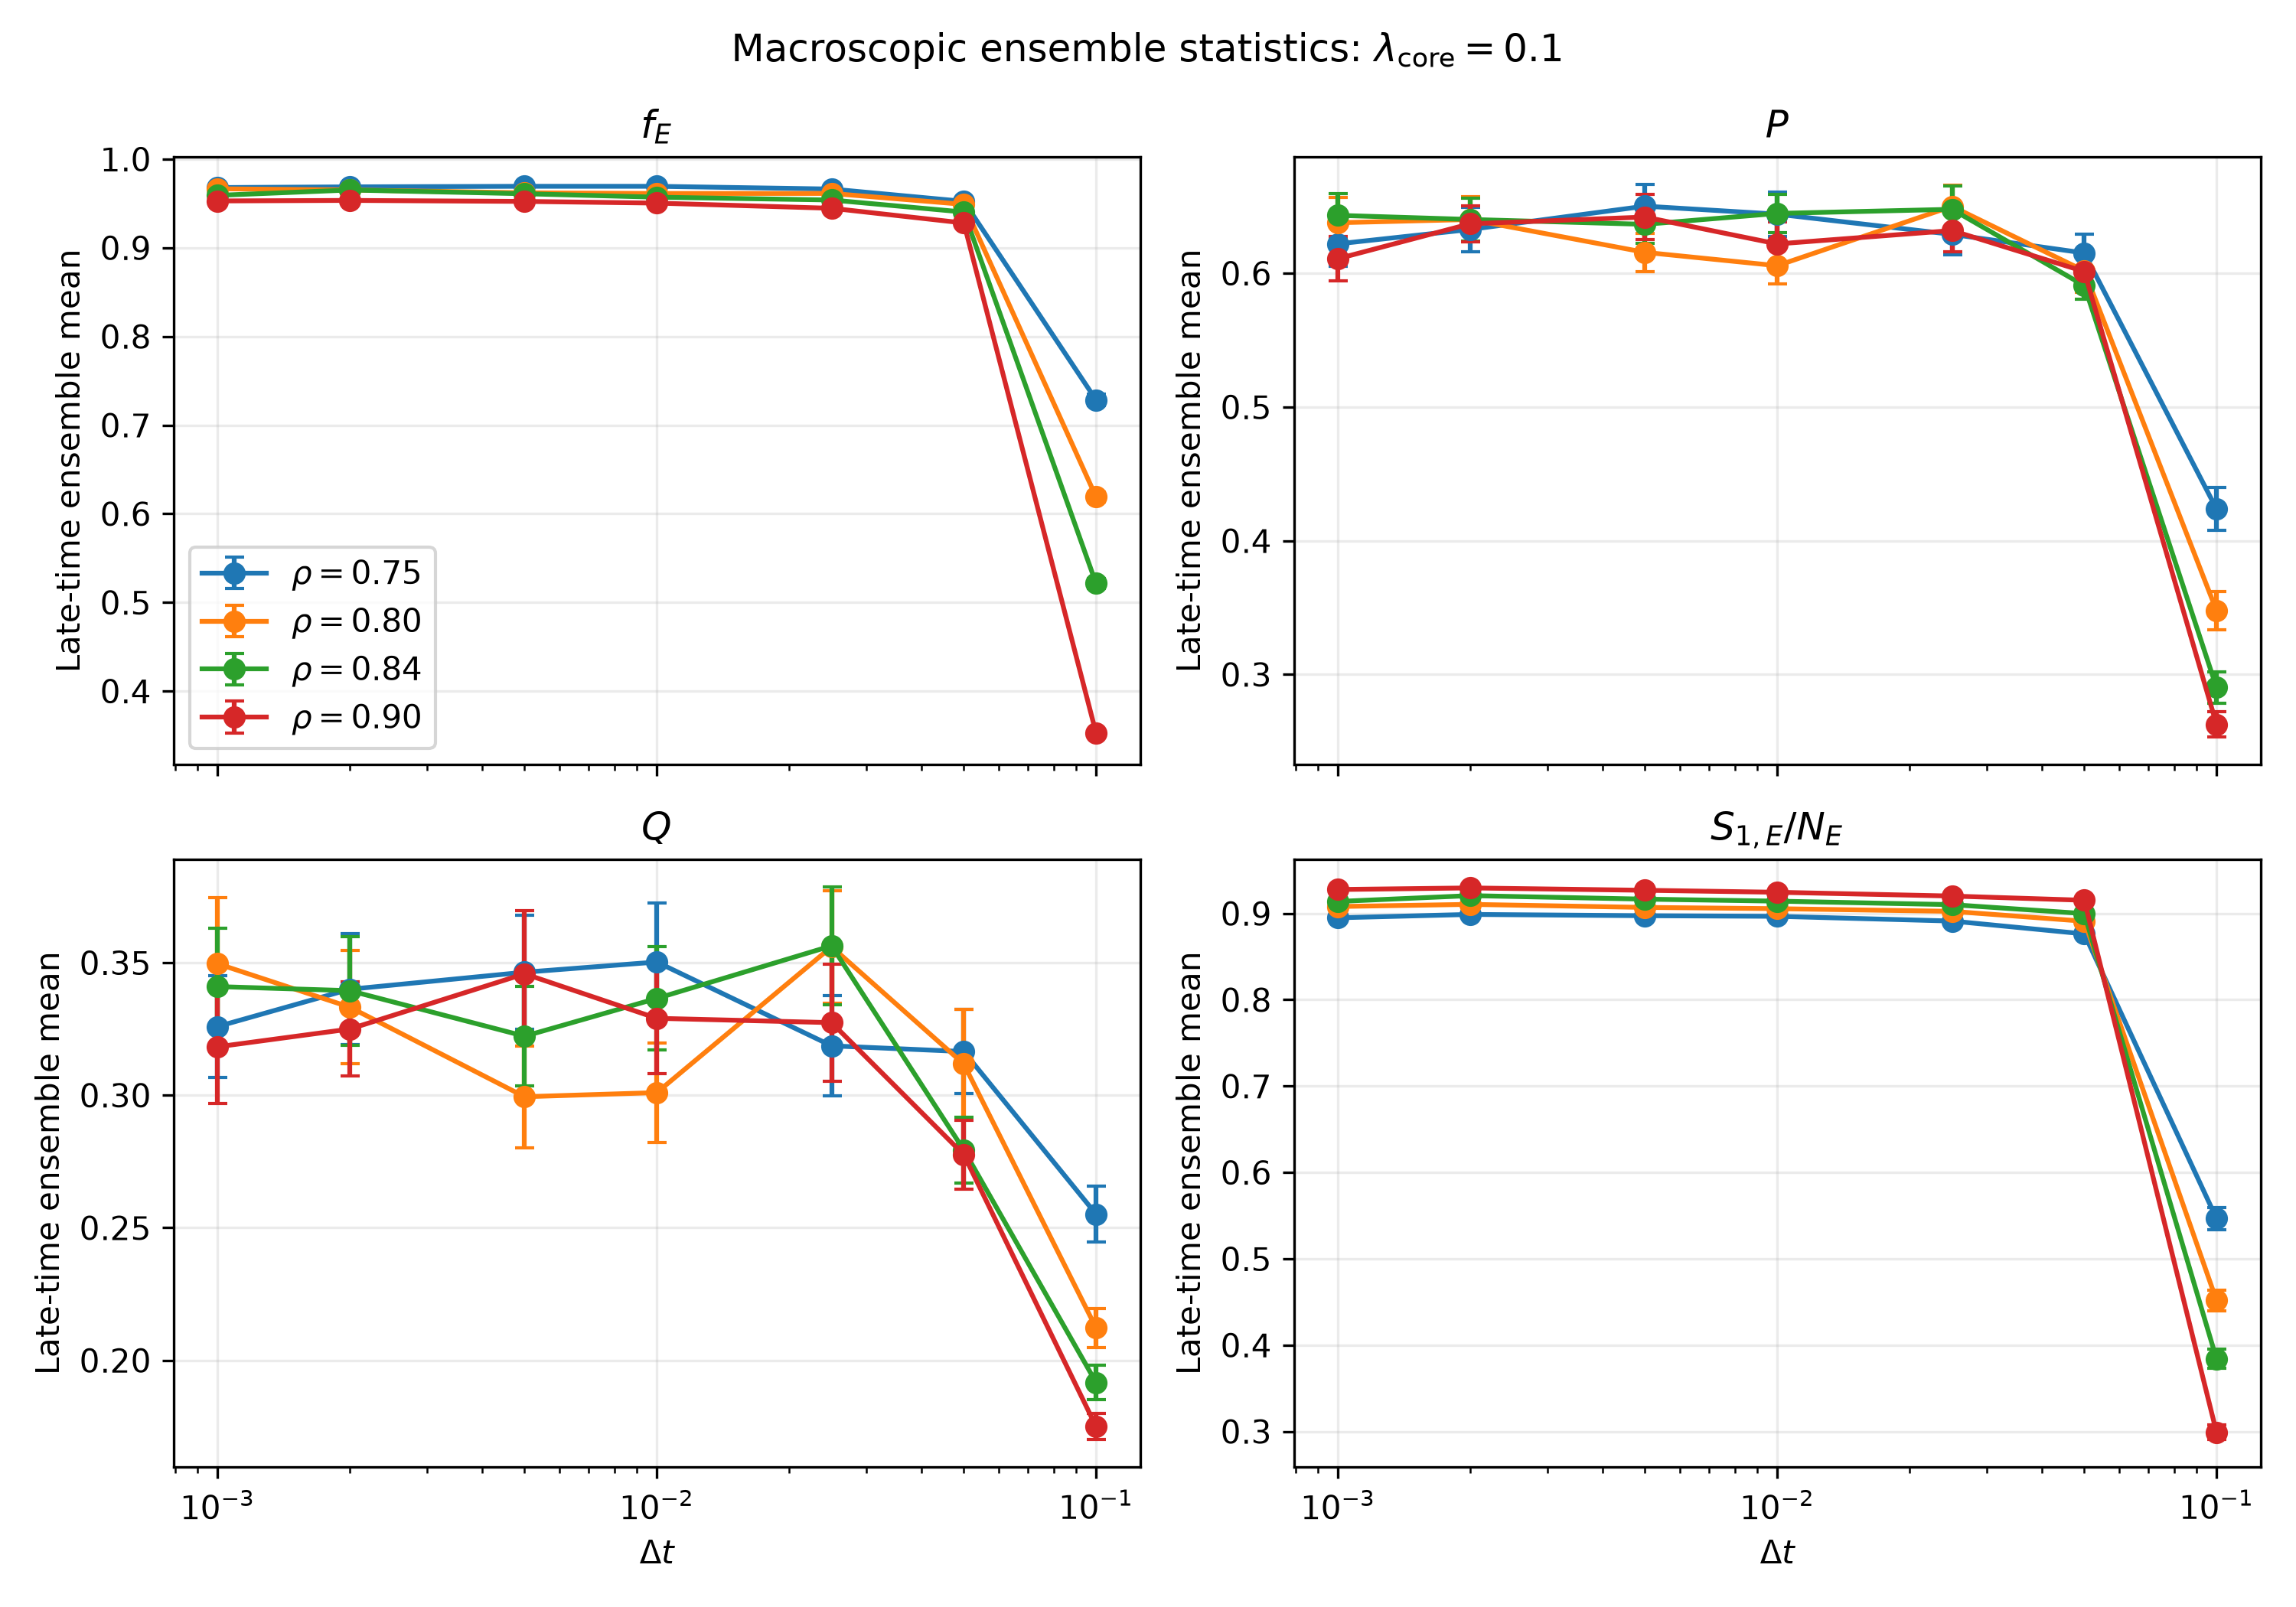
\includegraphics[width=\textwidth]
        {../figures/macro_ensemble_statistics_lambda_0.1.png}
        \caption{\(\lambda=0.1\).}
    \end{subfigure}
    \hfill
    \begin{subfigure}[t]{0.48\textwidth}
        \centering
        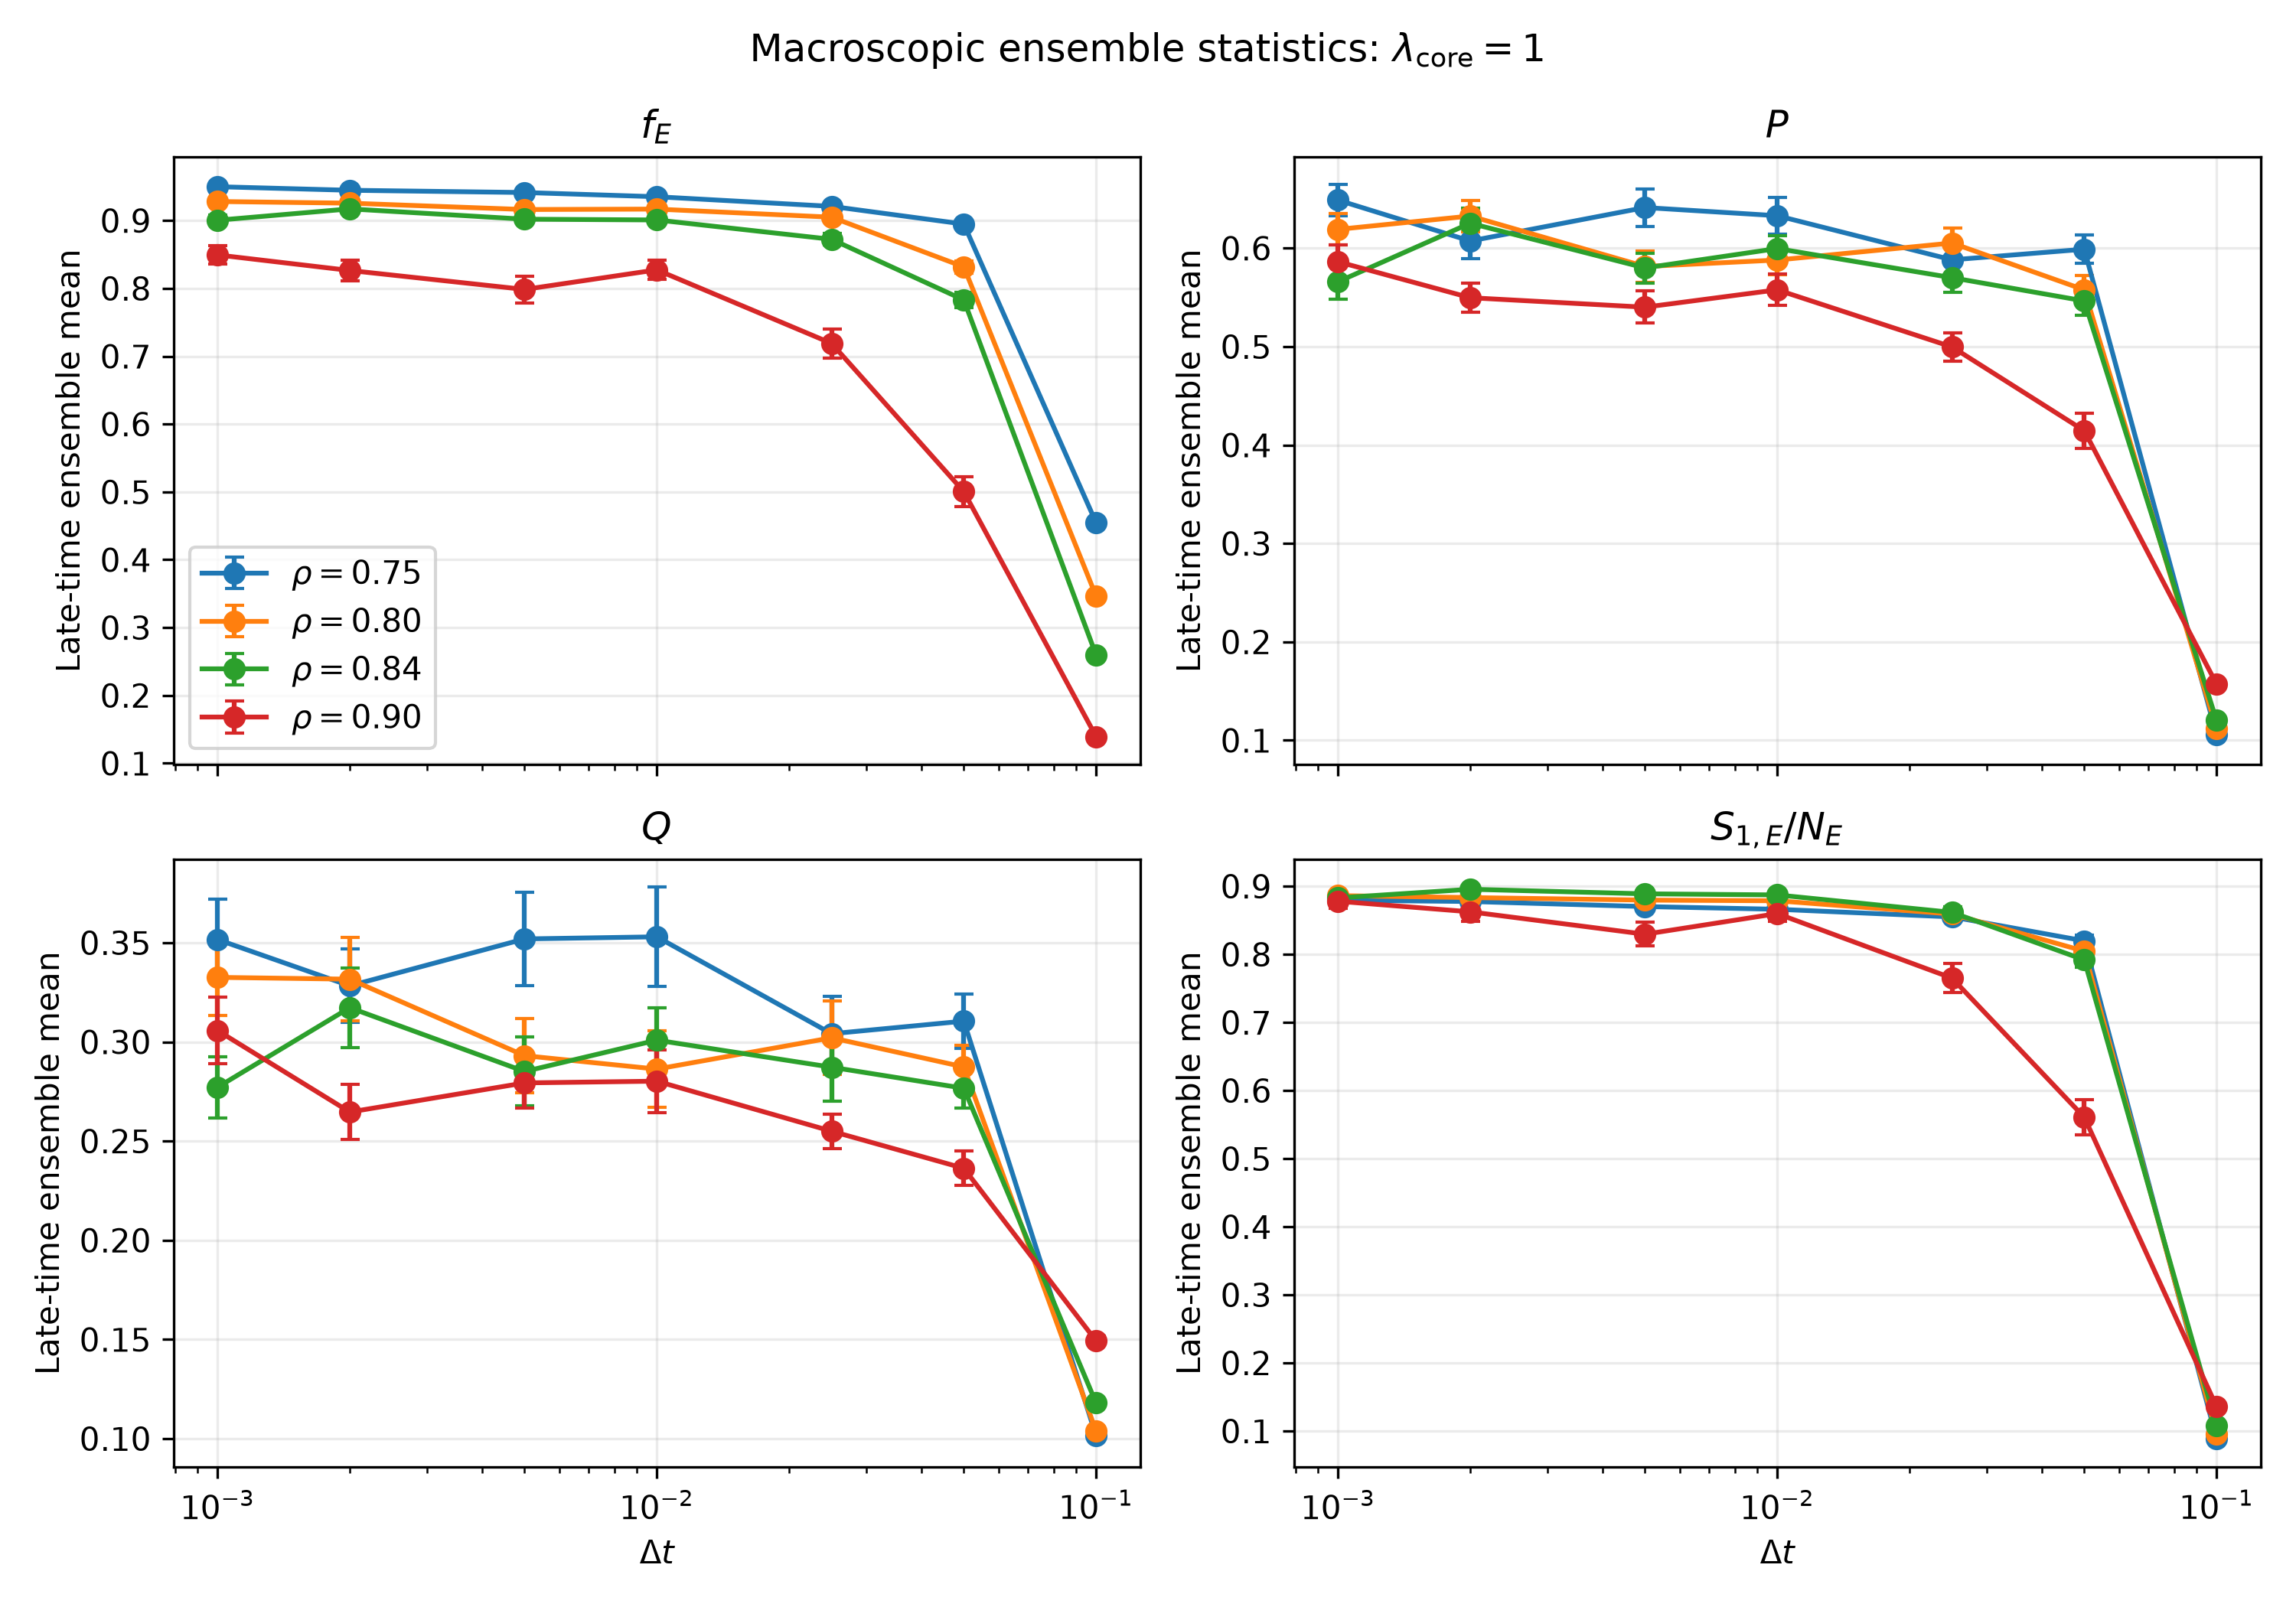
\includegraphics[width=\textwidth]
        {../figures/macro_ensemble_statistics_lambda_1.png}
        \caption{\(\lambda=1\).}
    \end{subfigure}
    \caption{
        Medias de ensamble de los observables macroscópicos en la ventana
        tardía, con error estándar entre realizaciones.
    }
    \label{fig:macro_stats}
\end{figure}

Para resumir la convergencia definimos, para cada observable \(X\),

\begin{equation}
\Delta_X(\Delta t)
=
\left|
\left\langle X\right\rangle_{\Delta t}
-
\left\langle X\right\rangle_{0.001}
\right|,
\end{equation}

y tomamos el mayor valor entre las cuatro densidades. Este diagnóstico se
muestra en la figura~\ref{fig:macro_conv}. La comparación confirma un plateau
de pequeños pasos y una separación progresiva al aumentar \(\Delta t\).
Para \(\lambda=1\), el máximo cambio de las medias de ensamble es
aproximadamente \(0.06\), \(0.05\) y \(0.05\) para
\(\Delta t=0.002,0.005\) y \(0.01\), respectivamente; aumenta a
\(\sim0.13\) para \(0.025\) y a \(\sim0.35\) para \(0.05\).

\begin{figure}[htbp]
    \centering
    \begin{subfigure}[t]{0.48\textwidth}
        \centering
        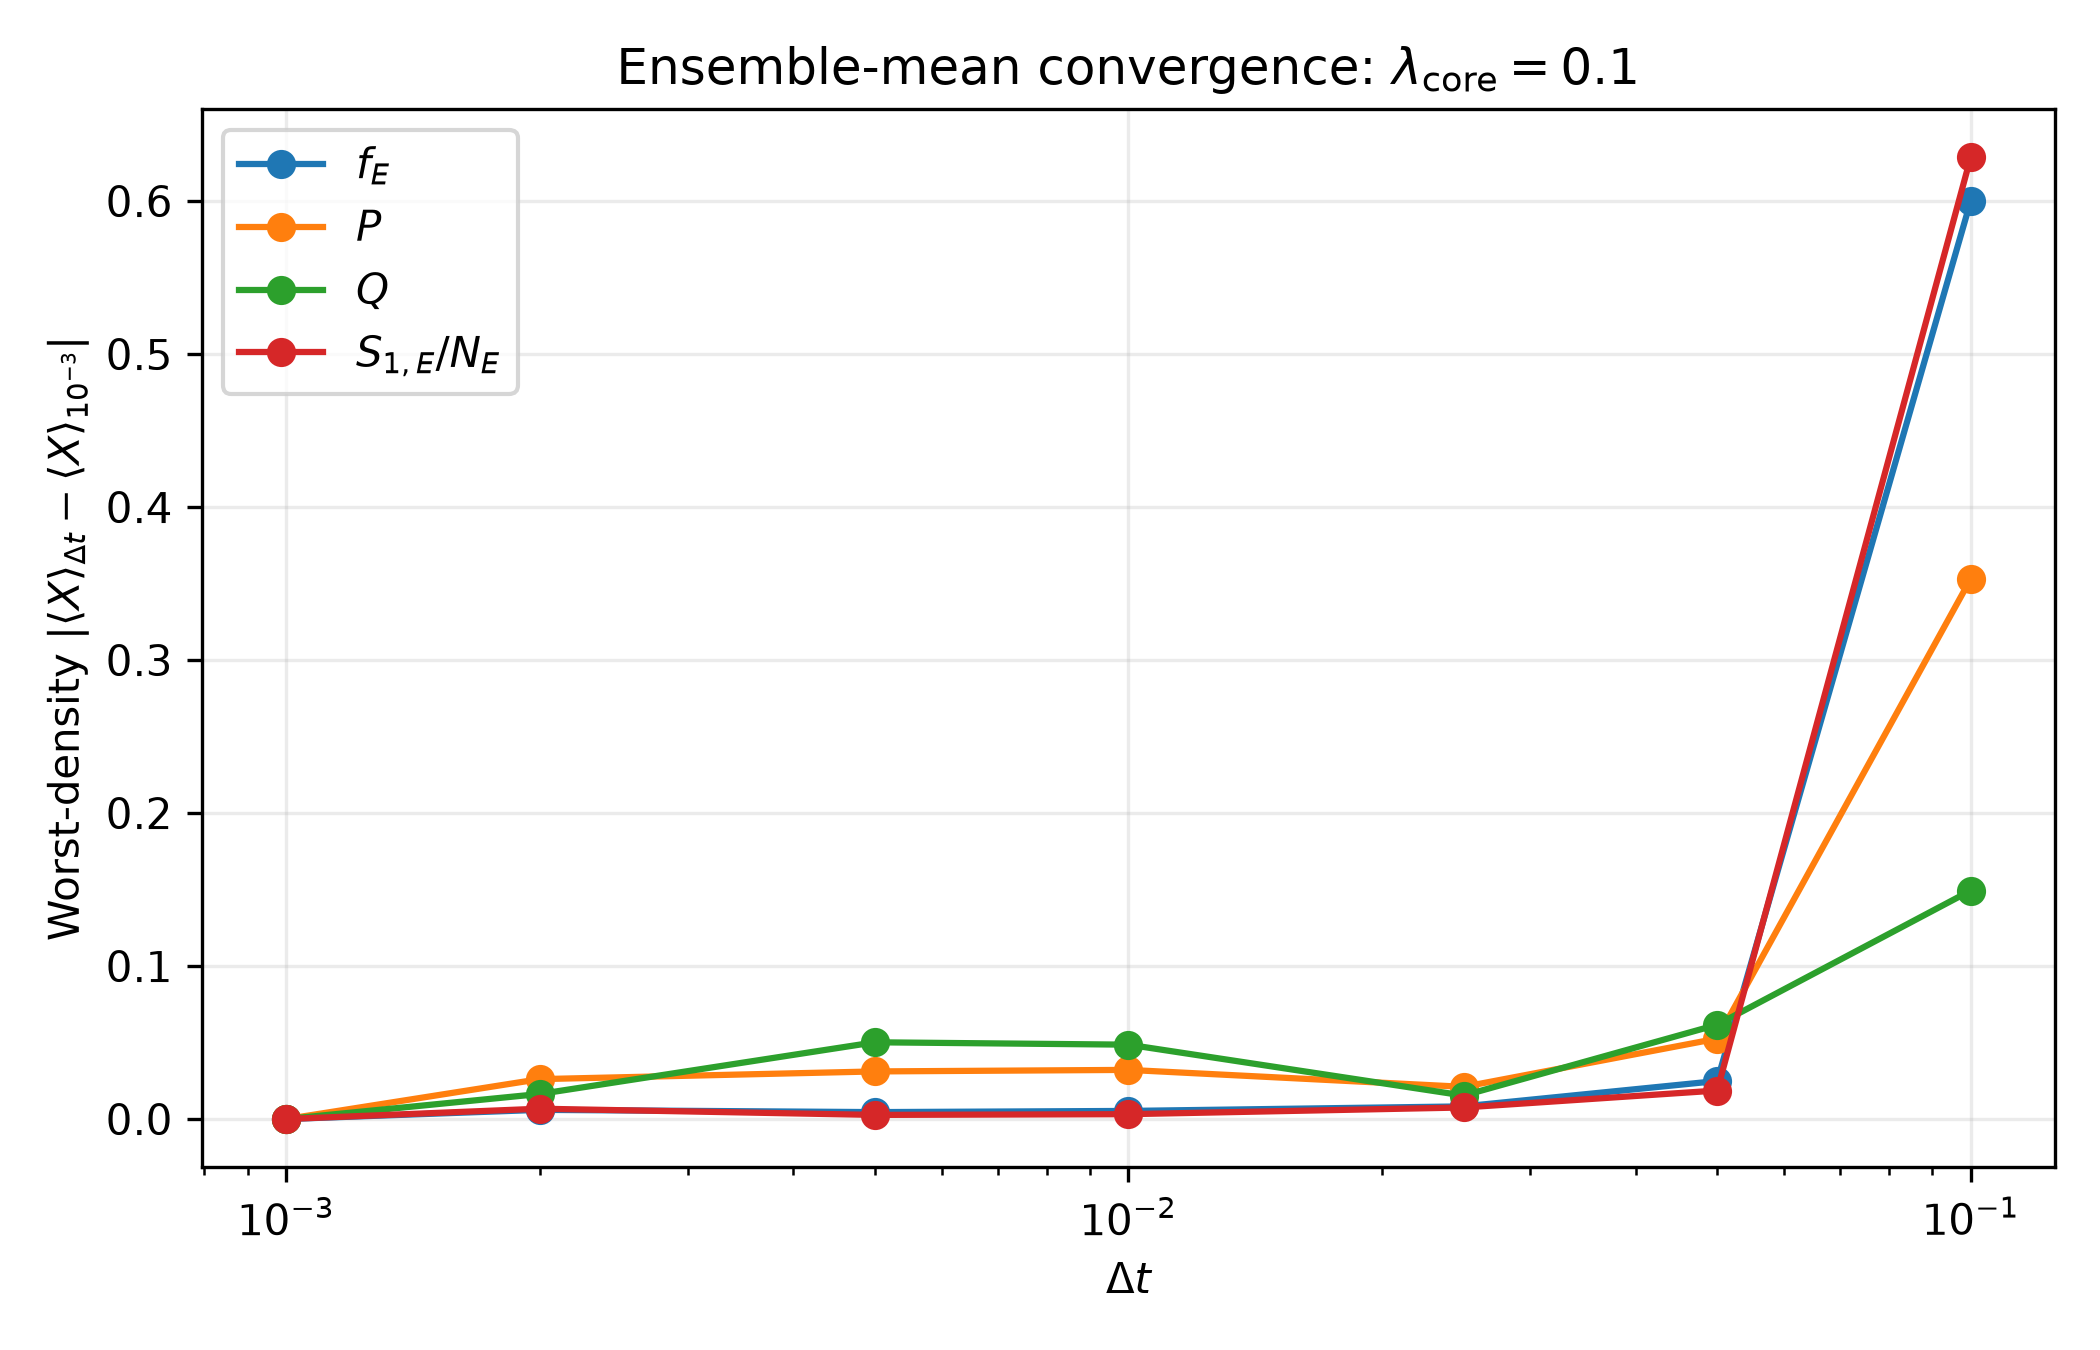
\includegraphics[width=\textwidth]
        {../figures/macro_ensemble_convergence_lambda_0.1.png}
        \caption{\(\lambda=0.1\).}
    \end{subfigure}
    \hfill
    \begin{subfigure}[t]{0.48\textwidth}
        \centering
        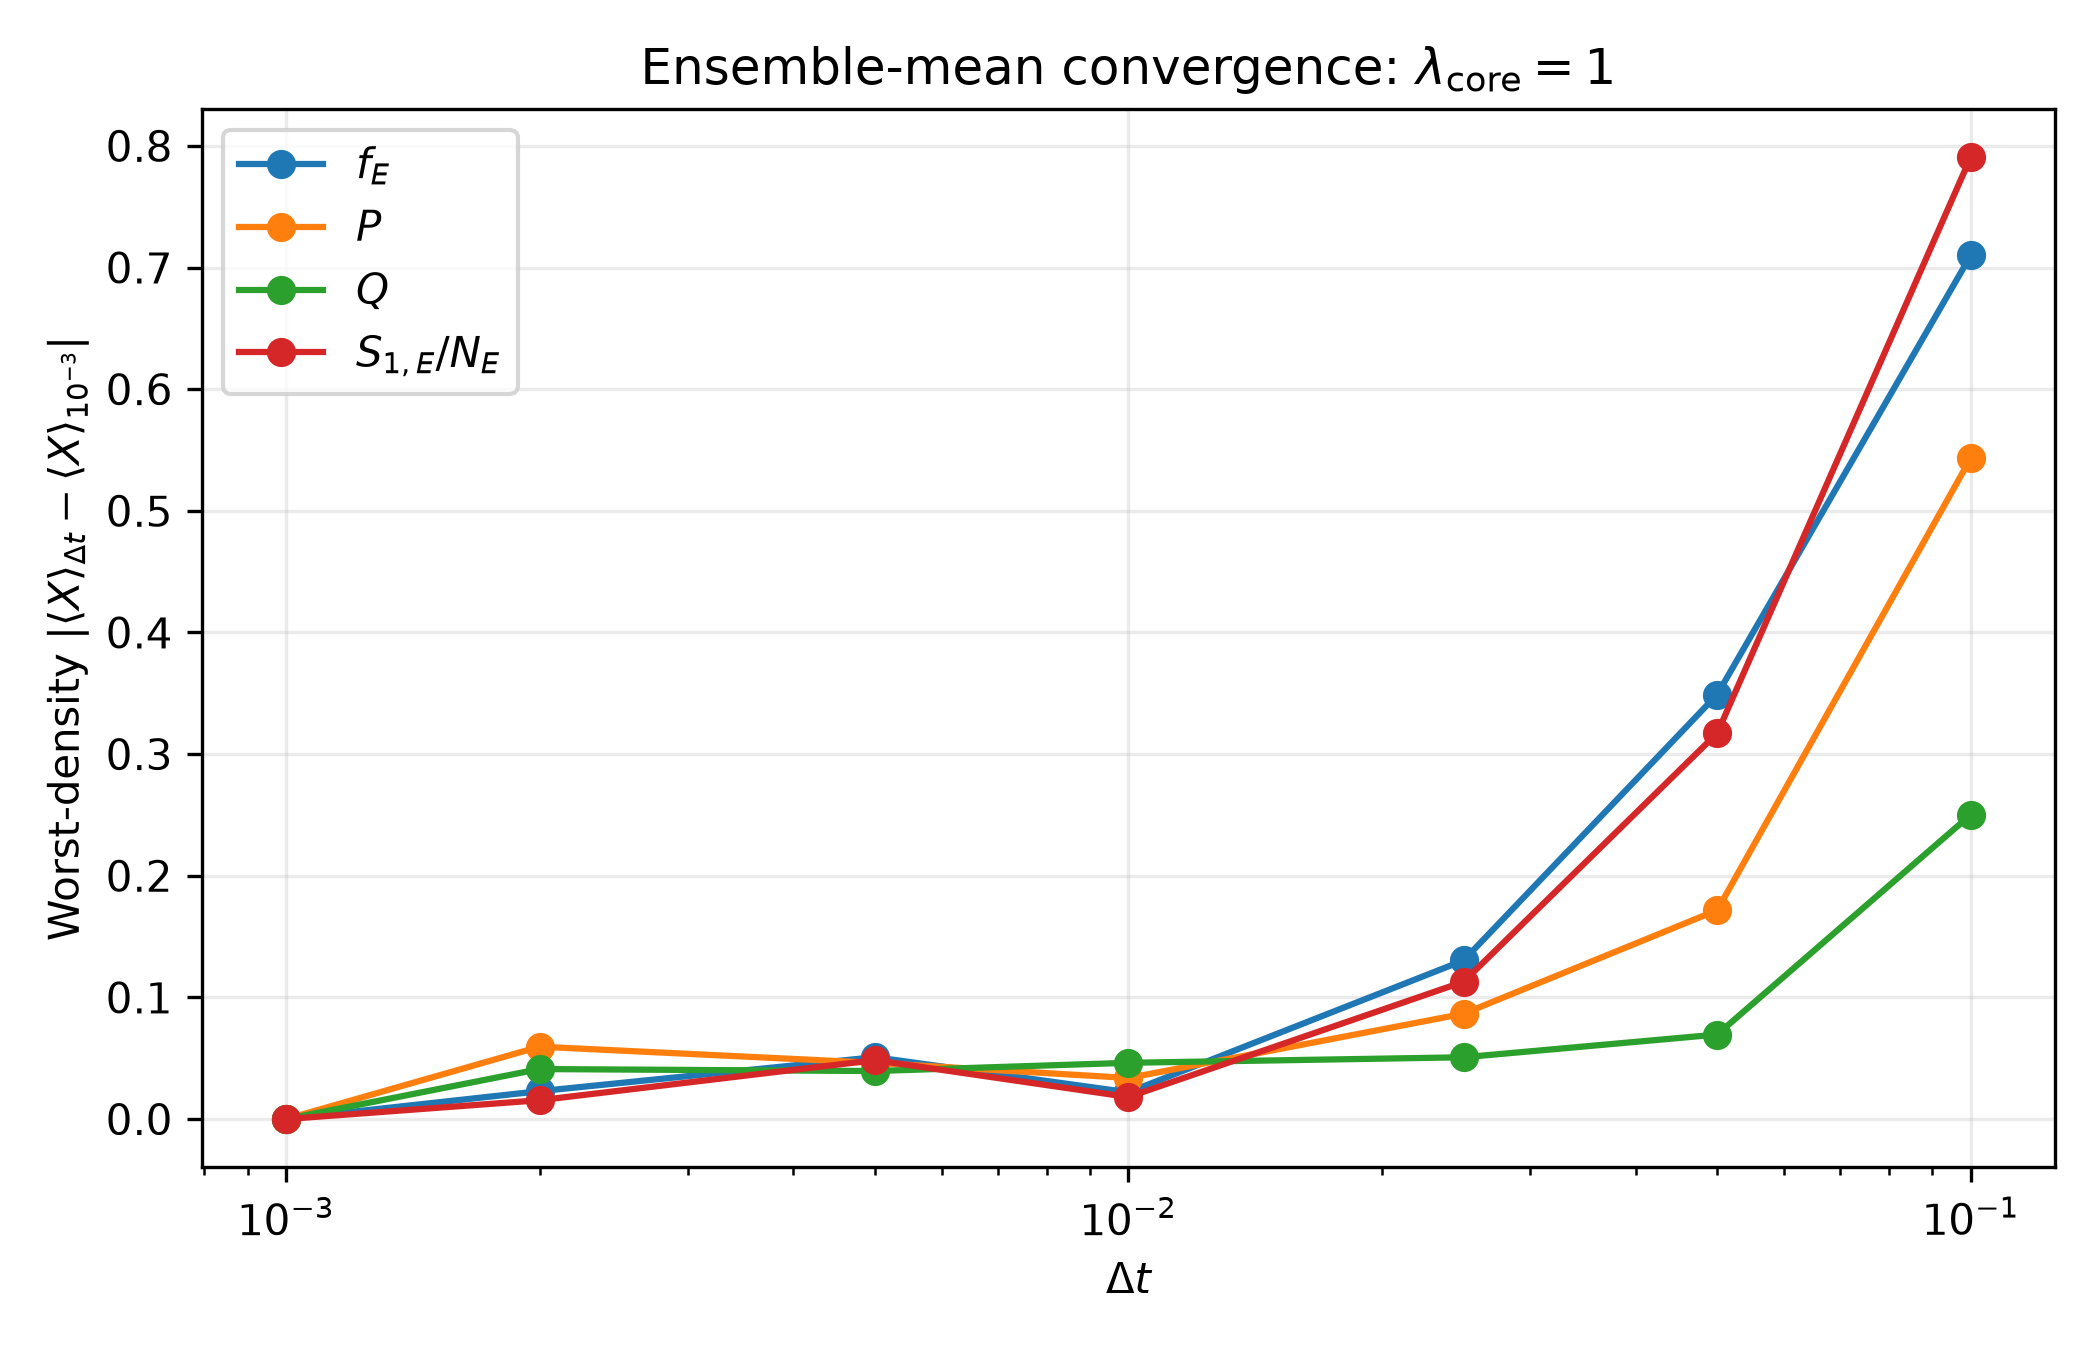
\includegraphics[width=\textwidth]
        {../figures/macro_ensemble_convergence_lambda_1.png}
        \caption{\(\lambda=1\).}
    \end{subfigure}
    \caption{
        Cambio de las medias de ensamble respecto de
        \(\Delta t=0.001\), tomando para cada observable el peor caso entre
        las densidades estudiadas.
    }
    \label{fig:macro_conv}
\end{figure}

\section{Superposiciones}

La regularización tiene como objetivo evitar que el sistema explore
configuraciones de superposición excesiva. Para cada realización analizamos la
cola de la máxima superposición normalizada \(\xi_{\max}\) durante la ventana
tardía.

La figura~\ref{fig:overlap} muestra que \(\lambda=1\) mantiene una cola de
superposición considerablemente menor que \(\lambda=0.1\). Para
\(\lambda=1\), el percentil 95 permanece aproximadamente constante y cercano a
\(0.79\) hasta \(\Delta t=0.01\). En \(\Delta t=0.025\) todavía no se observa
una inestabilidad severa, pero para \(\Delta t=0.05\) la cola crece de manera
clara y aparecen configuraciones más profundas.

\begin{figure}[htbp]
    \centering
    \begin{subfigure}[t]{0.48\textwidth}
        \centering
        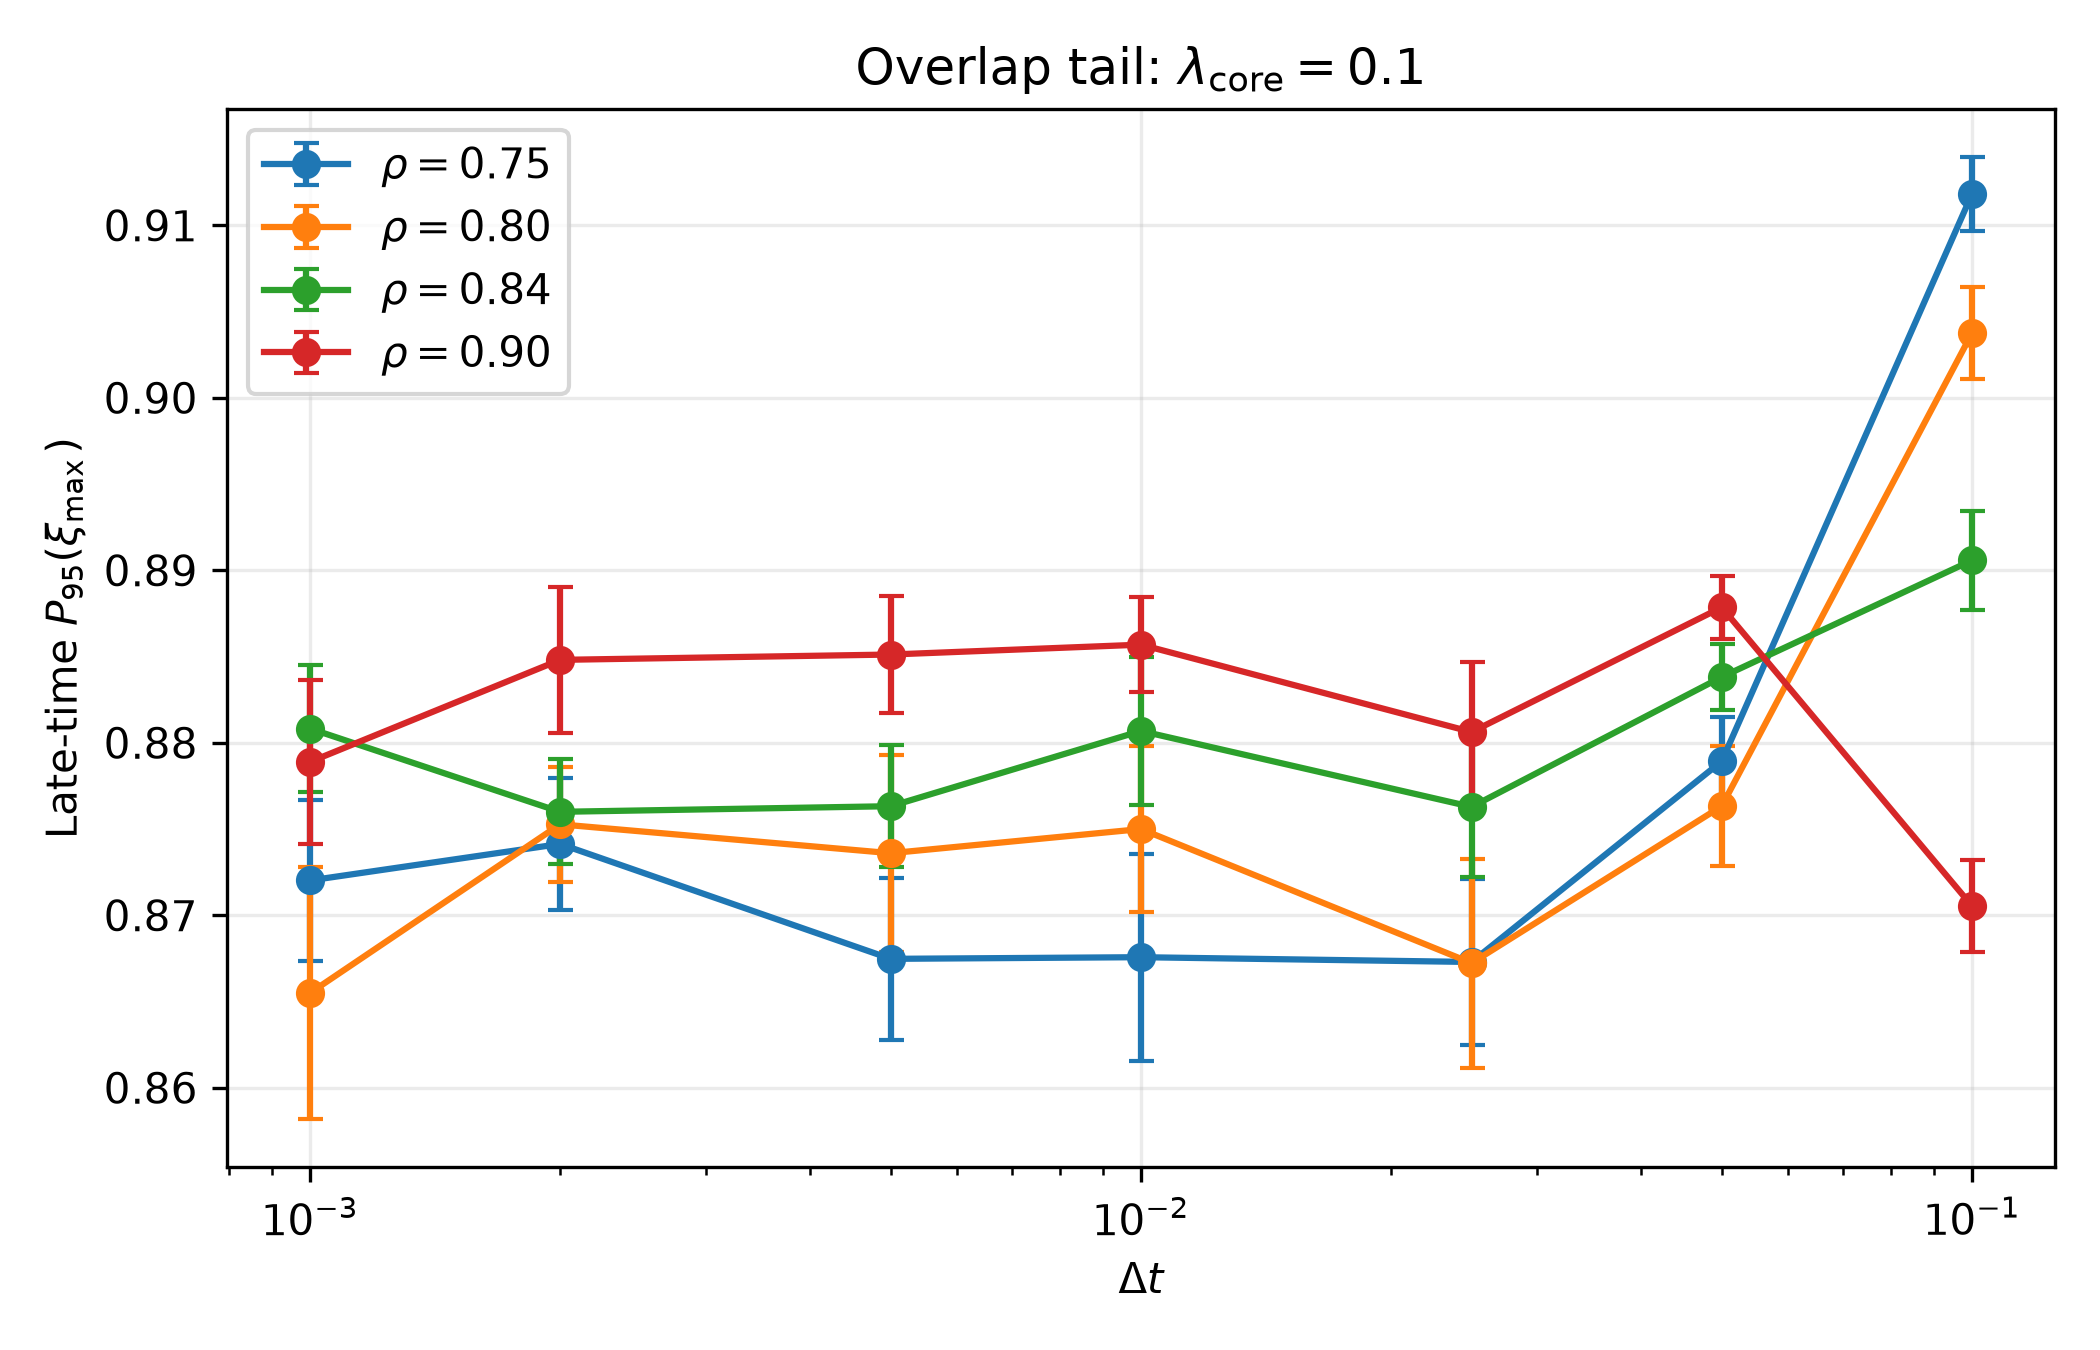
\includegraphics[width=\textwidth]
        {../figures/macro_ensemble_overlap_lambda_0.1.png}
        \caption{\(\lambda=0.1\).}
    \end{subfigure}
    \hfill
    \begin{subfigure}[t]{0.48\textwidth}
        \centering
        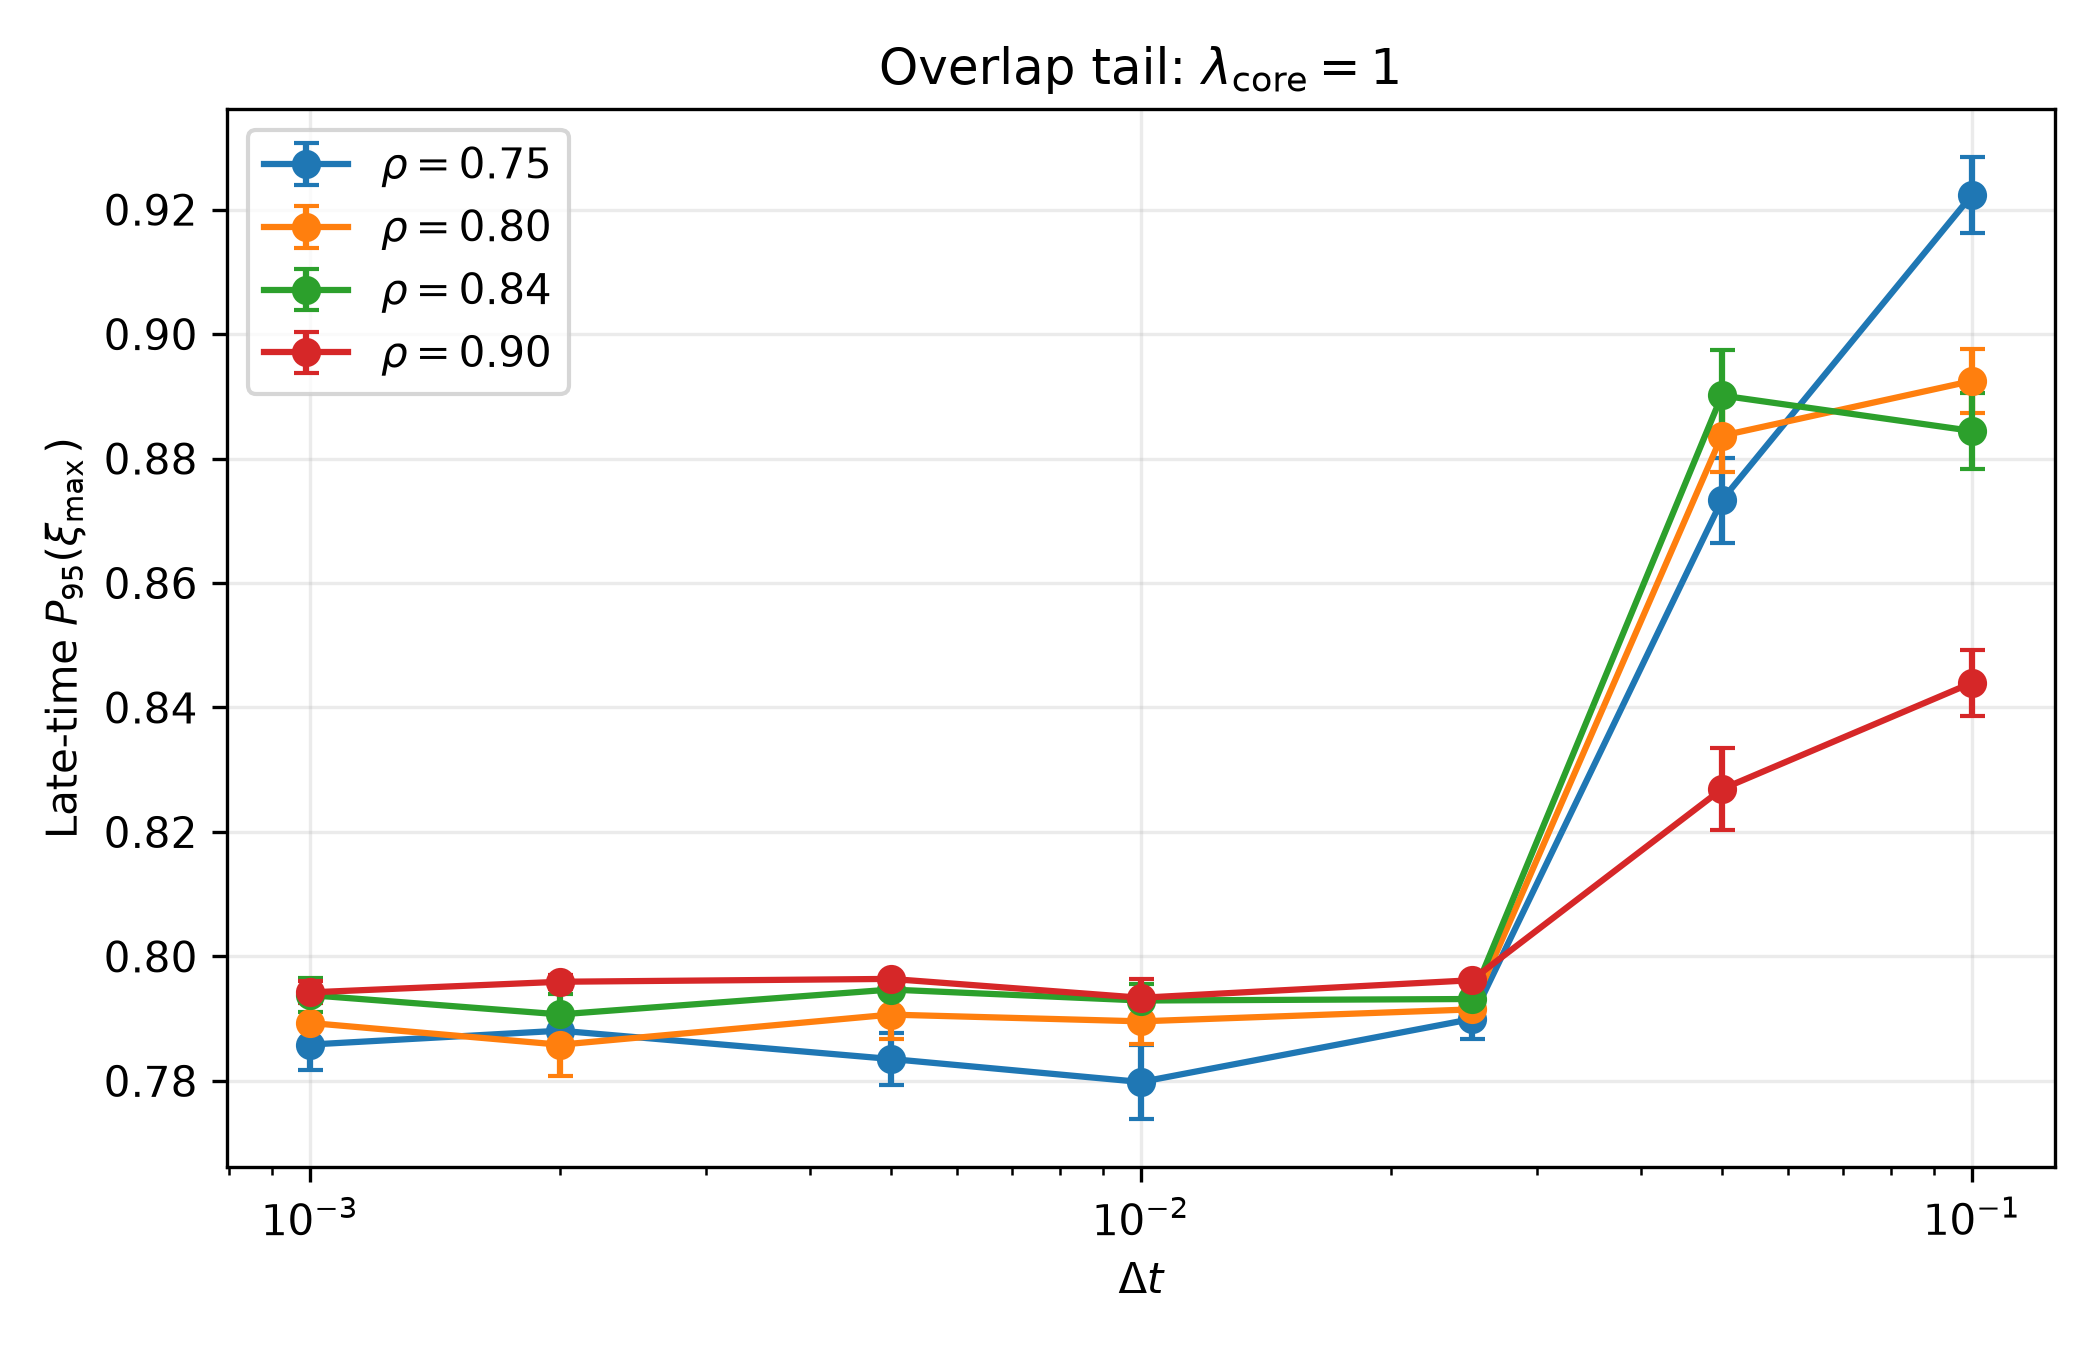
\includegraphics[width=\textwidth]
        {../figures/macro_ensemble_overlap_lambda_1.png}
        \caption{\(\lambda=1\).}
    \end{subfigure}
    \caption{
        Percentil 95 de la máxima superposición normalizada en la ventana
        tardía.
    }
    \label{fig:overlap}
\end{figure}

Esta diferencia también se refleja en la regla de seguridad de contracción.
En el régimen de pequeños pasos, con \(\lambda=0.1\) aproximadamente entre un
\(8\%\) y un \(11\%\) de las contracciones propuestas son rechazadas por
superposición, mientras que con \(\lambda=1\) la fracción es menor al
\(1\%\). Por lo tanto, el núcleo fuerte evita que la regla de seguridad tenga
que intervenir frecuentemente.

\section{Velocidades instantáneas}

También estudiamos la velocidad mecánica instantánea de cada célula. El
percentil 95 de su módulo se muestra en la figura~\ref{fig:speed_tail}. Para
\(\lambda=1\), esta cola permanece aproximadamente en el mismo régimen hasta
\(\Delta t\simeq0.025\); para pasos mayores comienza a crecer y el máximo de
velocidad presenta una desviación mucho más marcada.

\begin{figure}[htbp]
    \centering
    \begin{subfigure}[t]{0.48\textwidth}
        \centering
        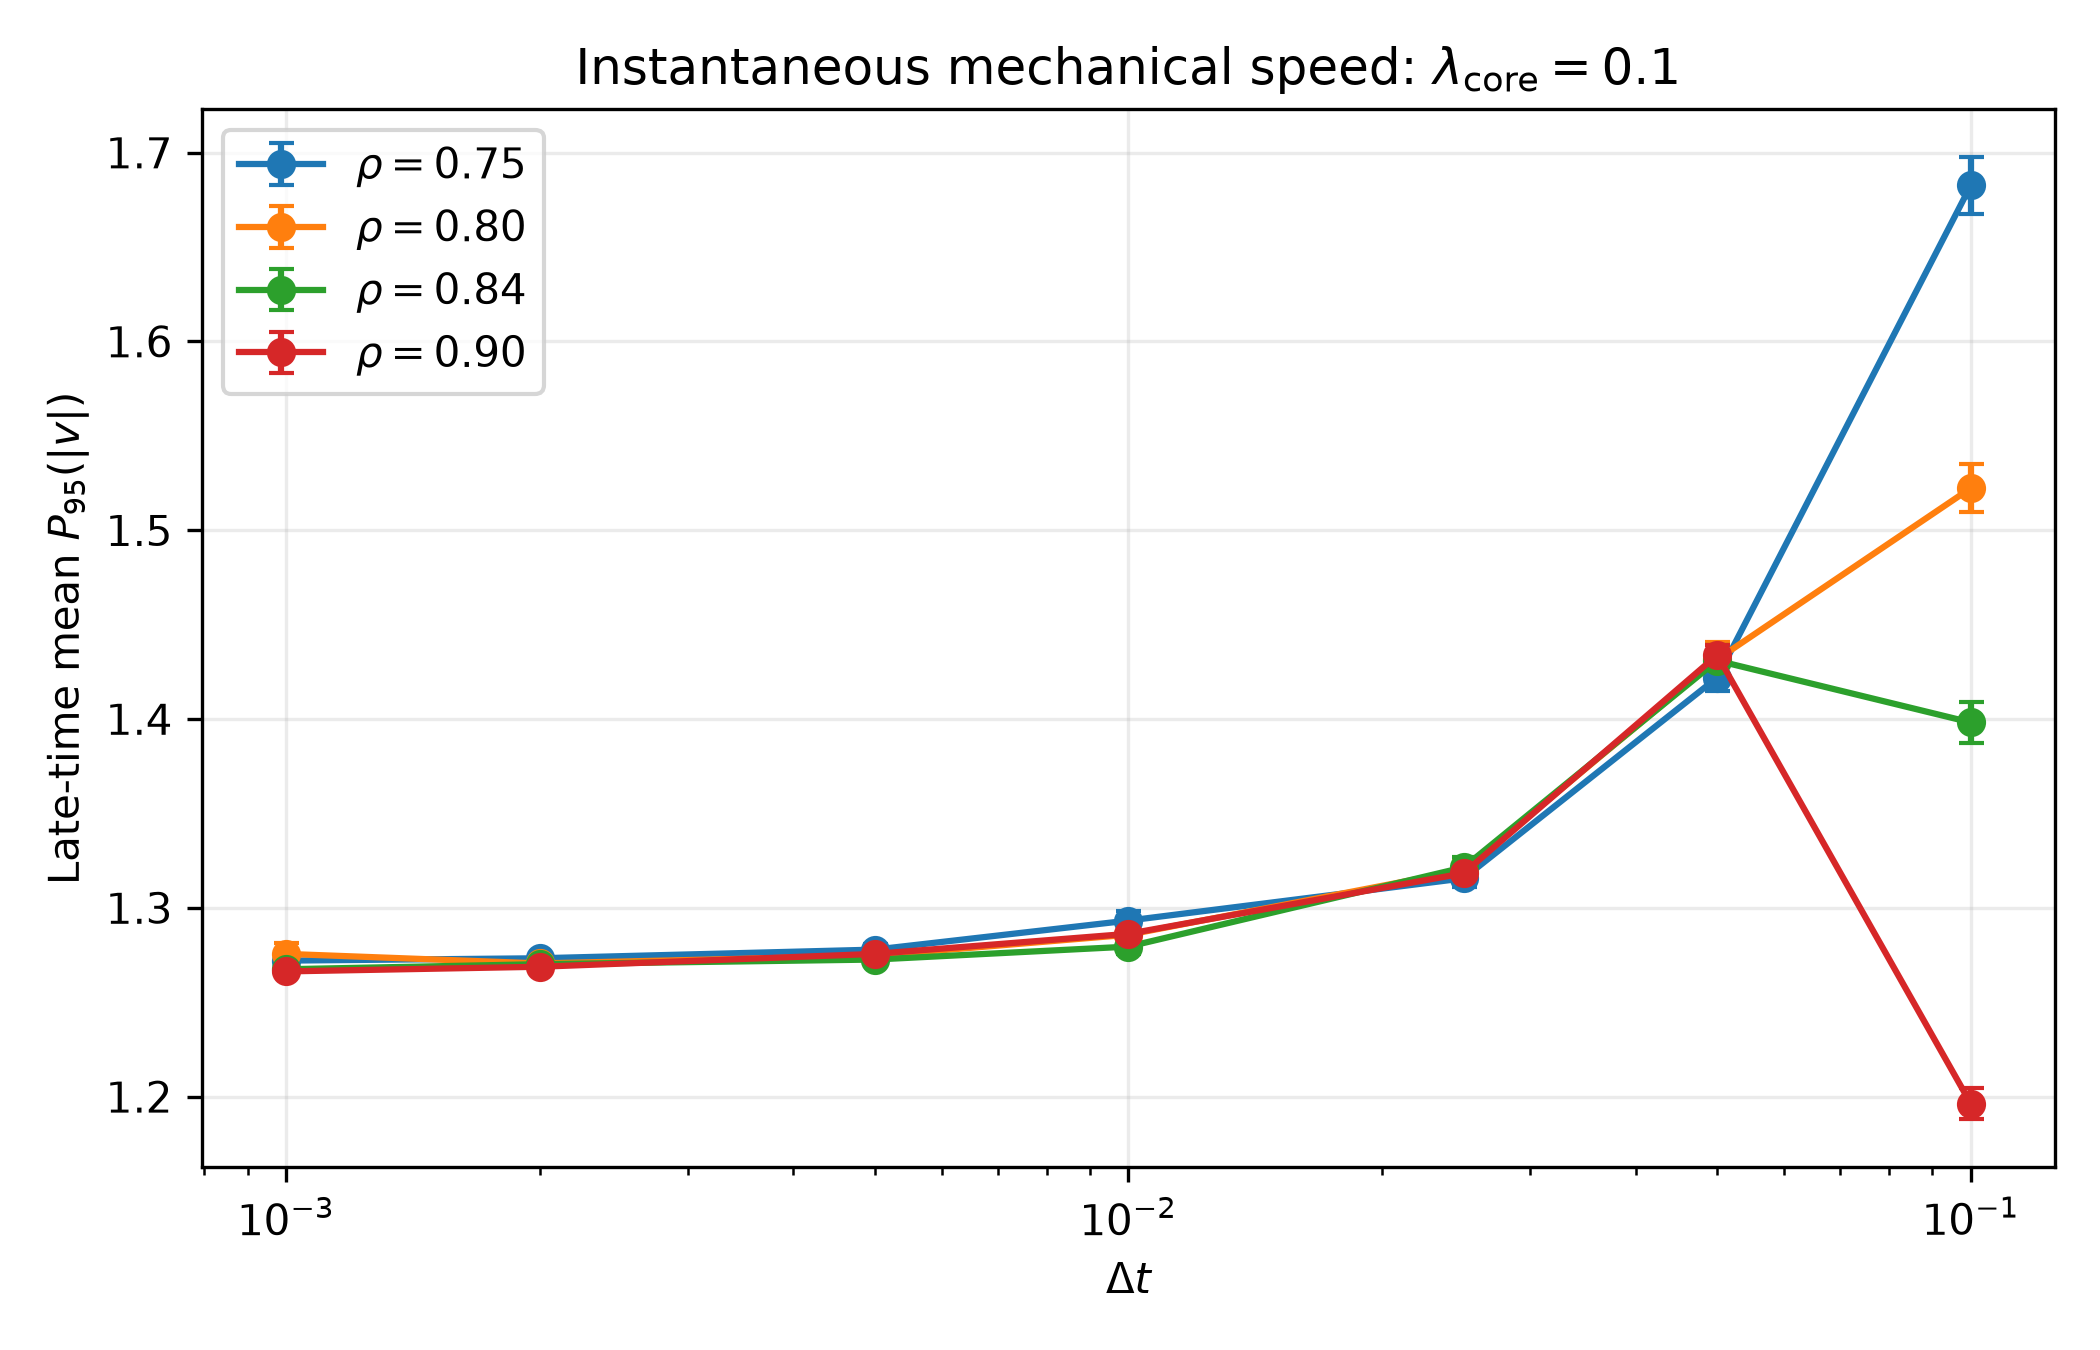
\includegraphics[width=\textwidth]
        {../figures/macro_ensemble_speed_lambda_0.1.png}
        \caption{\(\lambda=0.1\).}
    \end{subfigure}
    \hfill
    \begin{subfigure}[t]{0.48\textwidth}
        \centering
        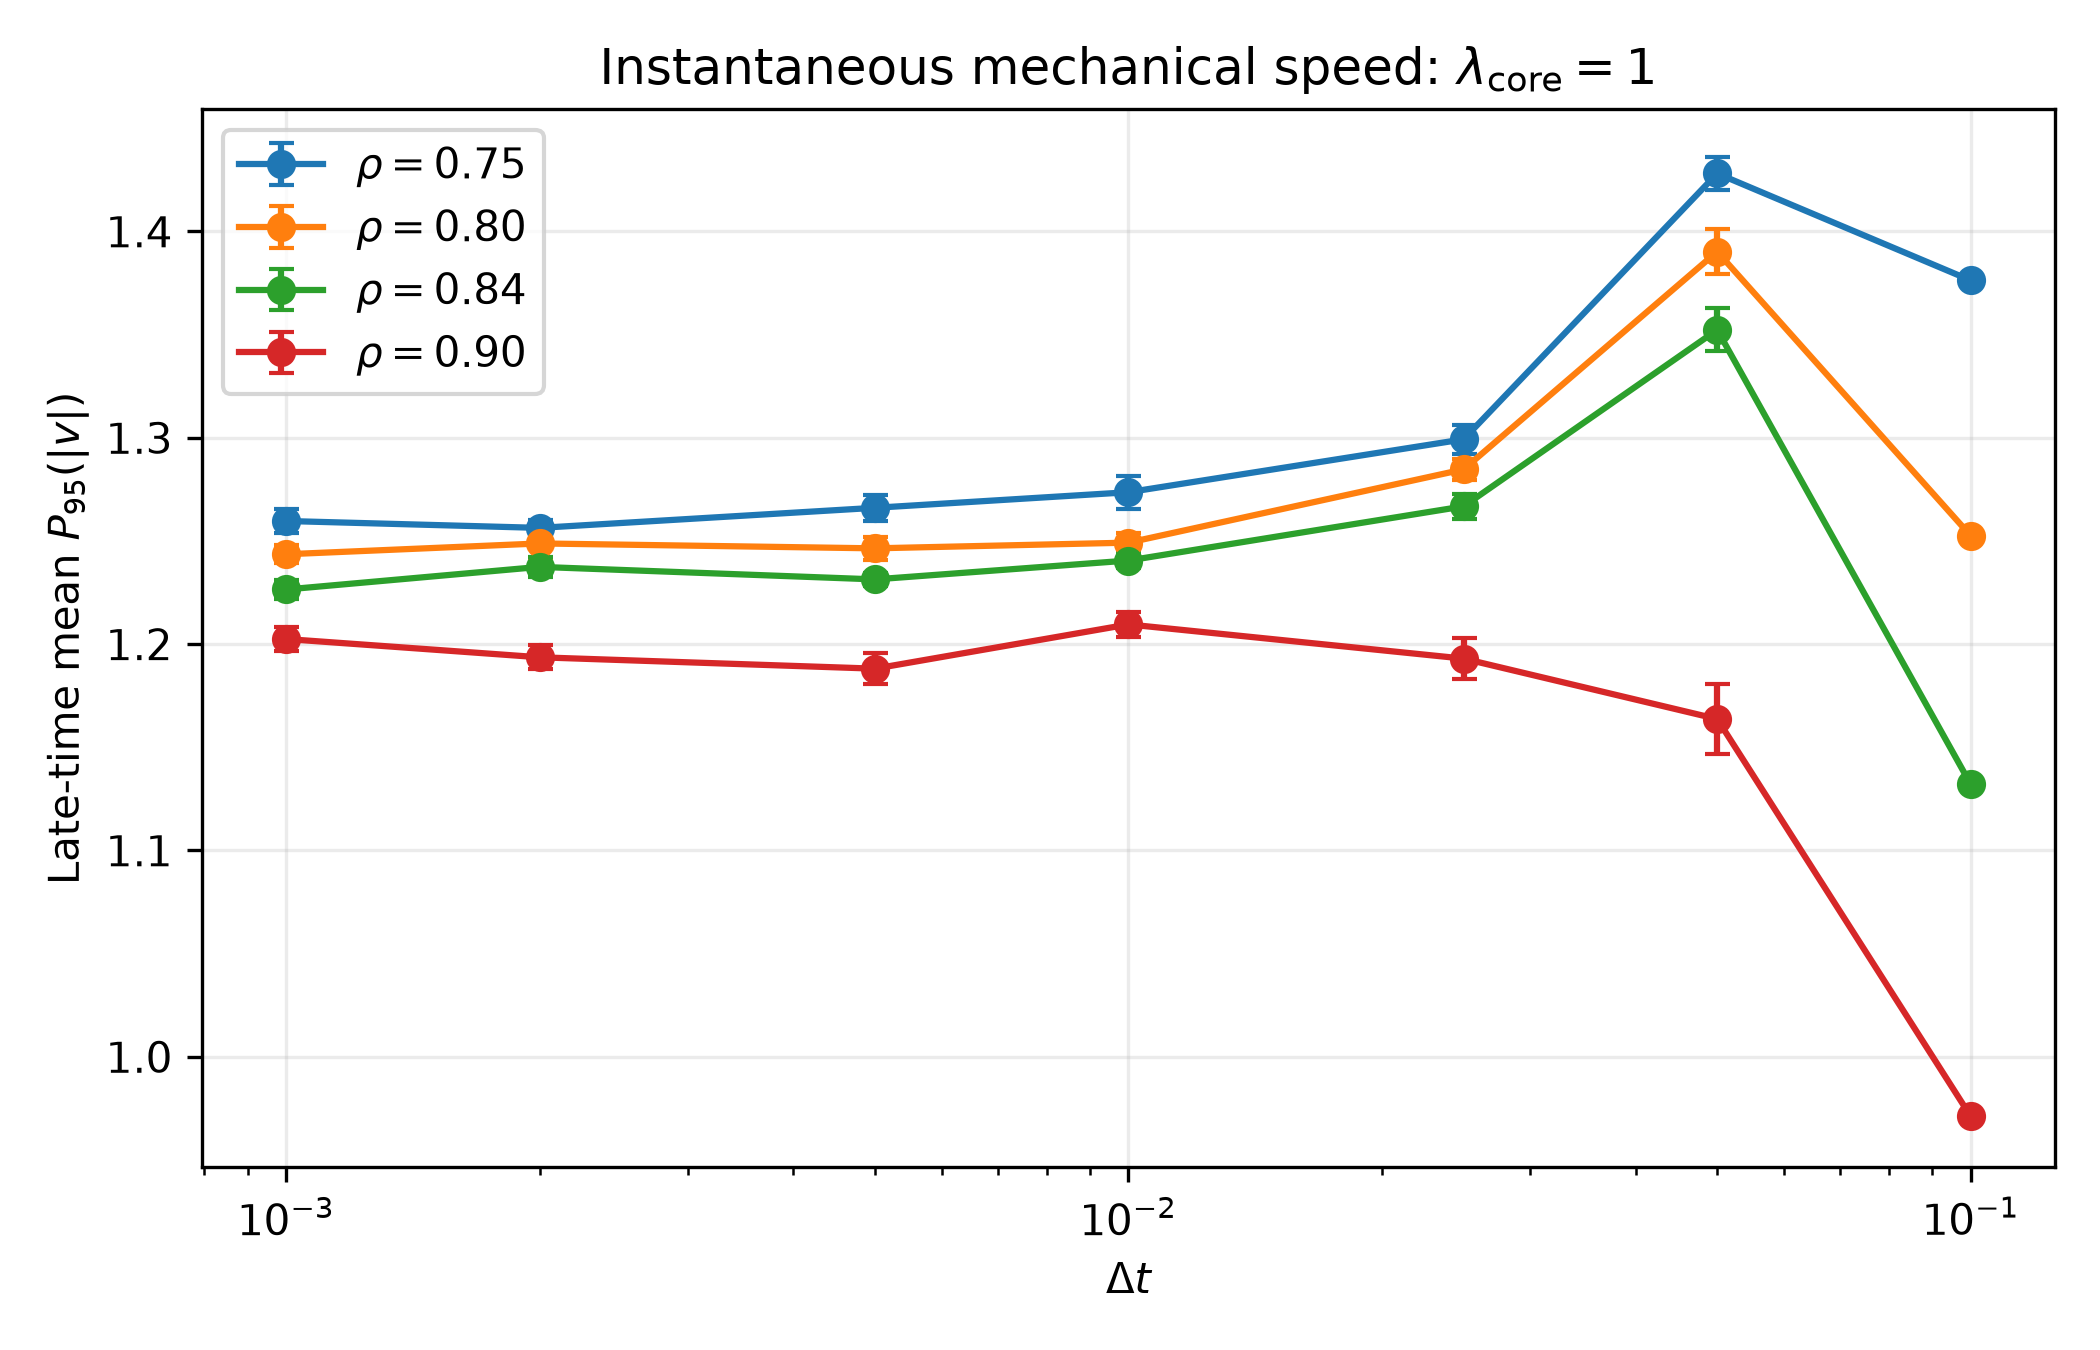
\includegraphics[width=\textwidth]
        {../figures/macro_ensemble_speed_lambda_1.png}
        \caption{\(\lambda=1\).}
    \end{subfigure}
    \caption{
        Percentil 95 del módulo de la velocidad instantánea en la ventana
        tardía.
    }
    \label{fig:speed_tail}
\end{figure}

Que el percentil 95 sea ligeramente mayor que uno no implica una aceleración
colectiva no física. La velocidad intrínseca \(v_0=1\) corresponde a una
célula elongada aislada, mientras que la velocidad total incluye además el
término mecánico debido a las interacciones. Localmente, las fuerzas pueden
acelerar algunas células y frenar o desviar otras.

Para verificar que la cola rápida no corresponde a una aceleración sistemática
del conjunto, en la figura~\ref{fig:mean_speed} mostramos la velocidad
instantánea media. Esta permanece por debajo de \(v_0=1\): las interacciones,
en promedio, dificultan el movimiento autopropulsado aunque algunas células
puedan tener velocidades instantáneas mayores que uno.

\begin{figure}[htbp]
    \centering
    \begin{subfigure}[t]{0.48\textwidth}
        \centering
        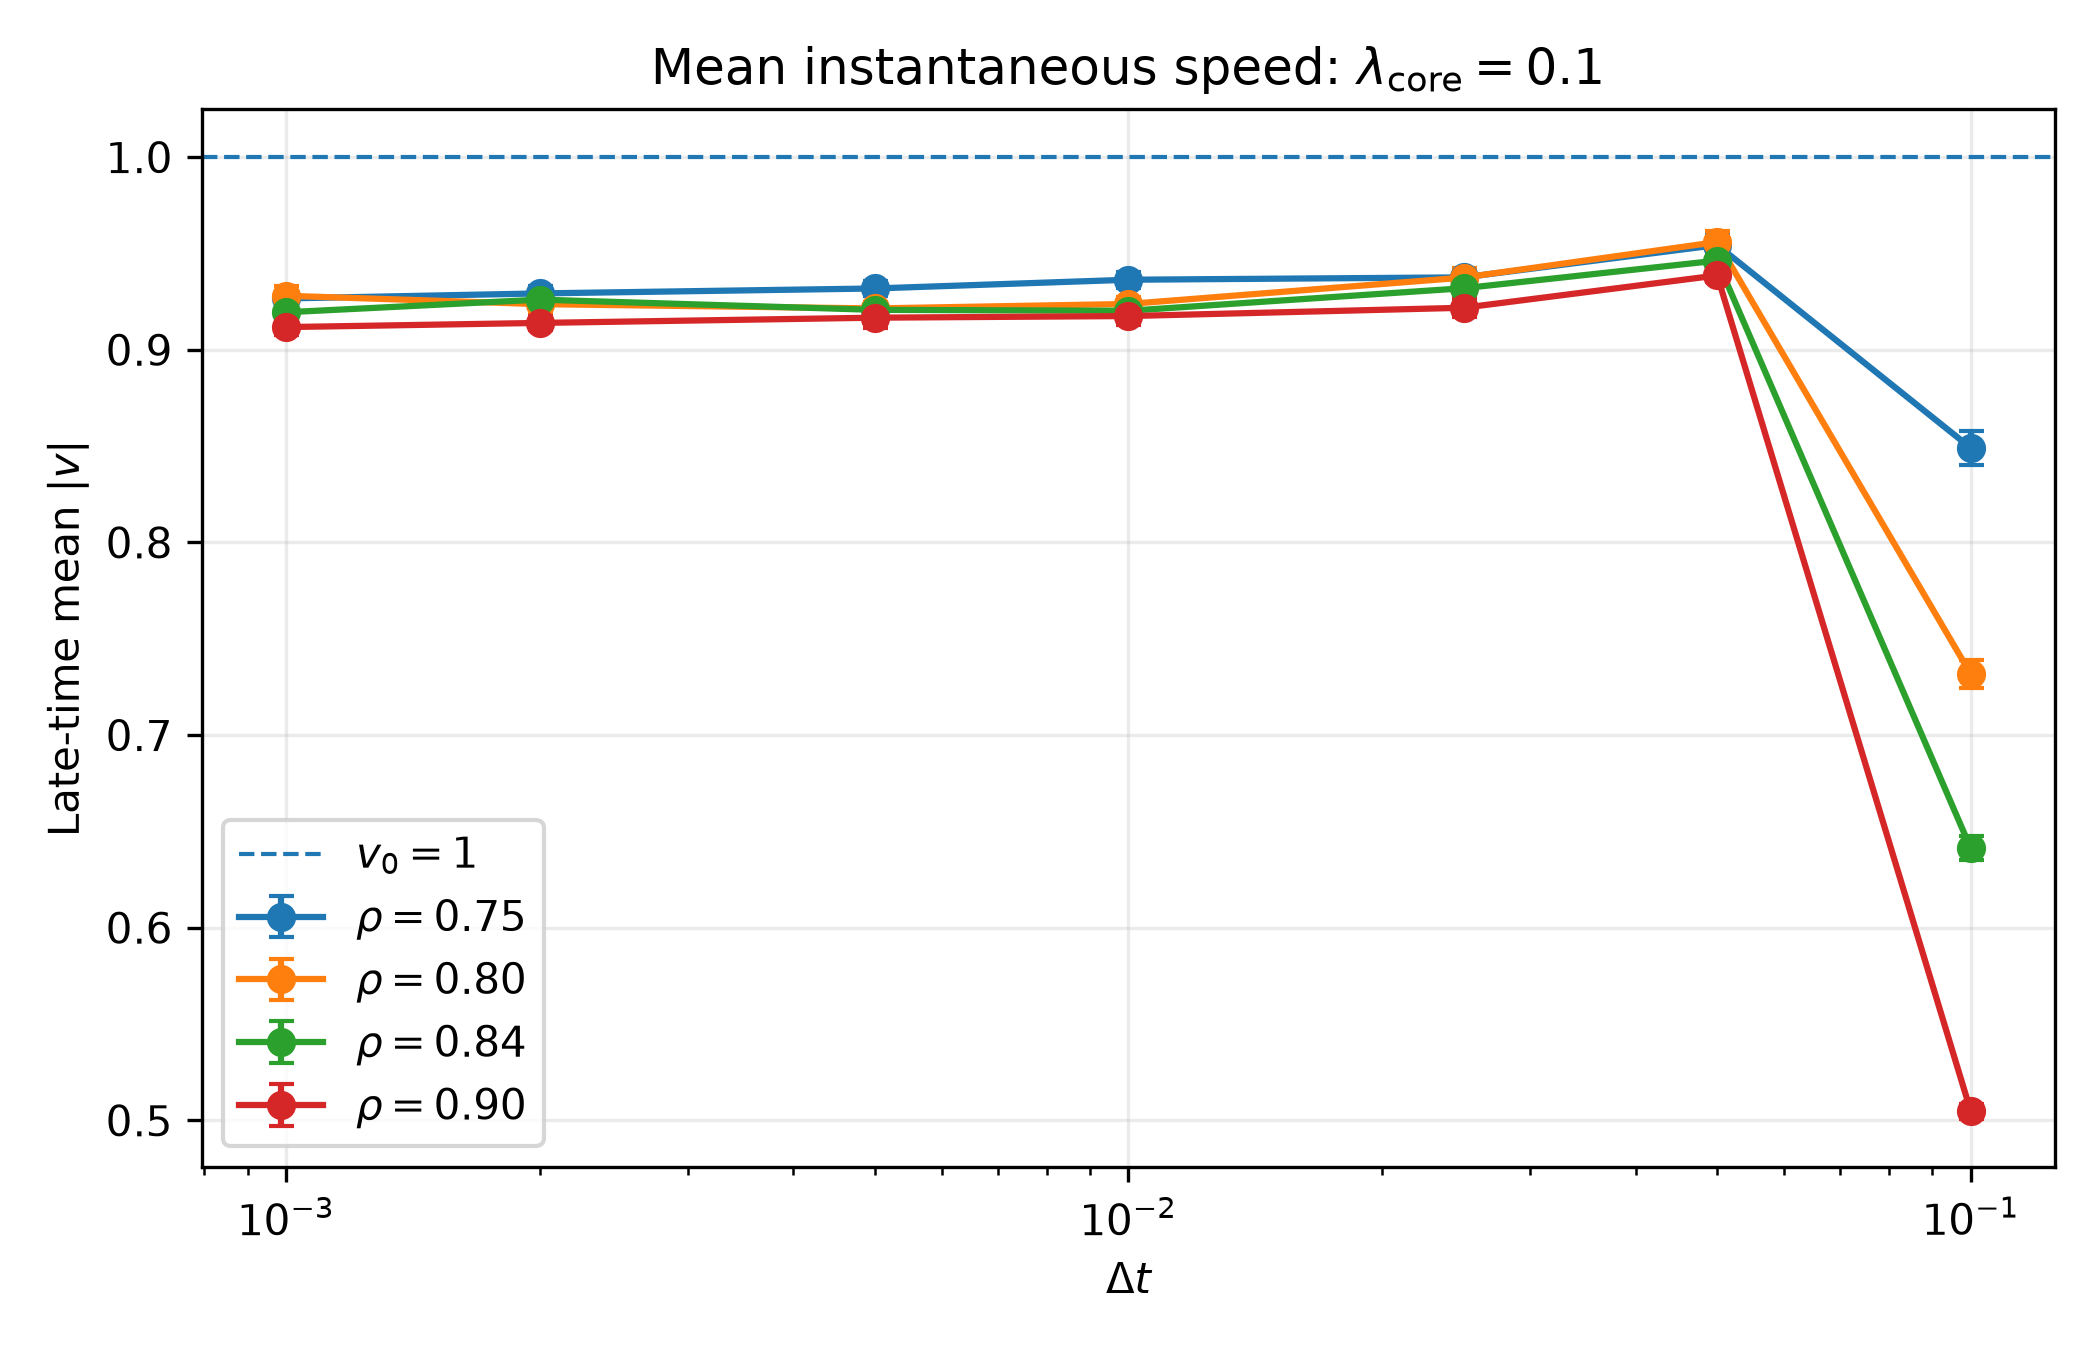
\includegraphics[width=\textwidth]
        {../figures/macro_ensemble_mean_speed_lambda_0.1.png}
        \caption{\(\lambda=0.1\).}
    \end{subfigure}
    \hfill
    \begin{subfigure}[t]{0.48\textwidth}
        \centering
        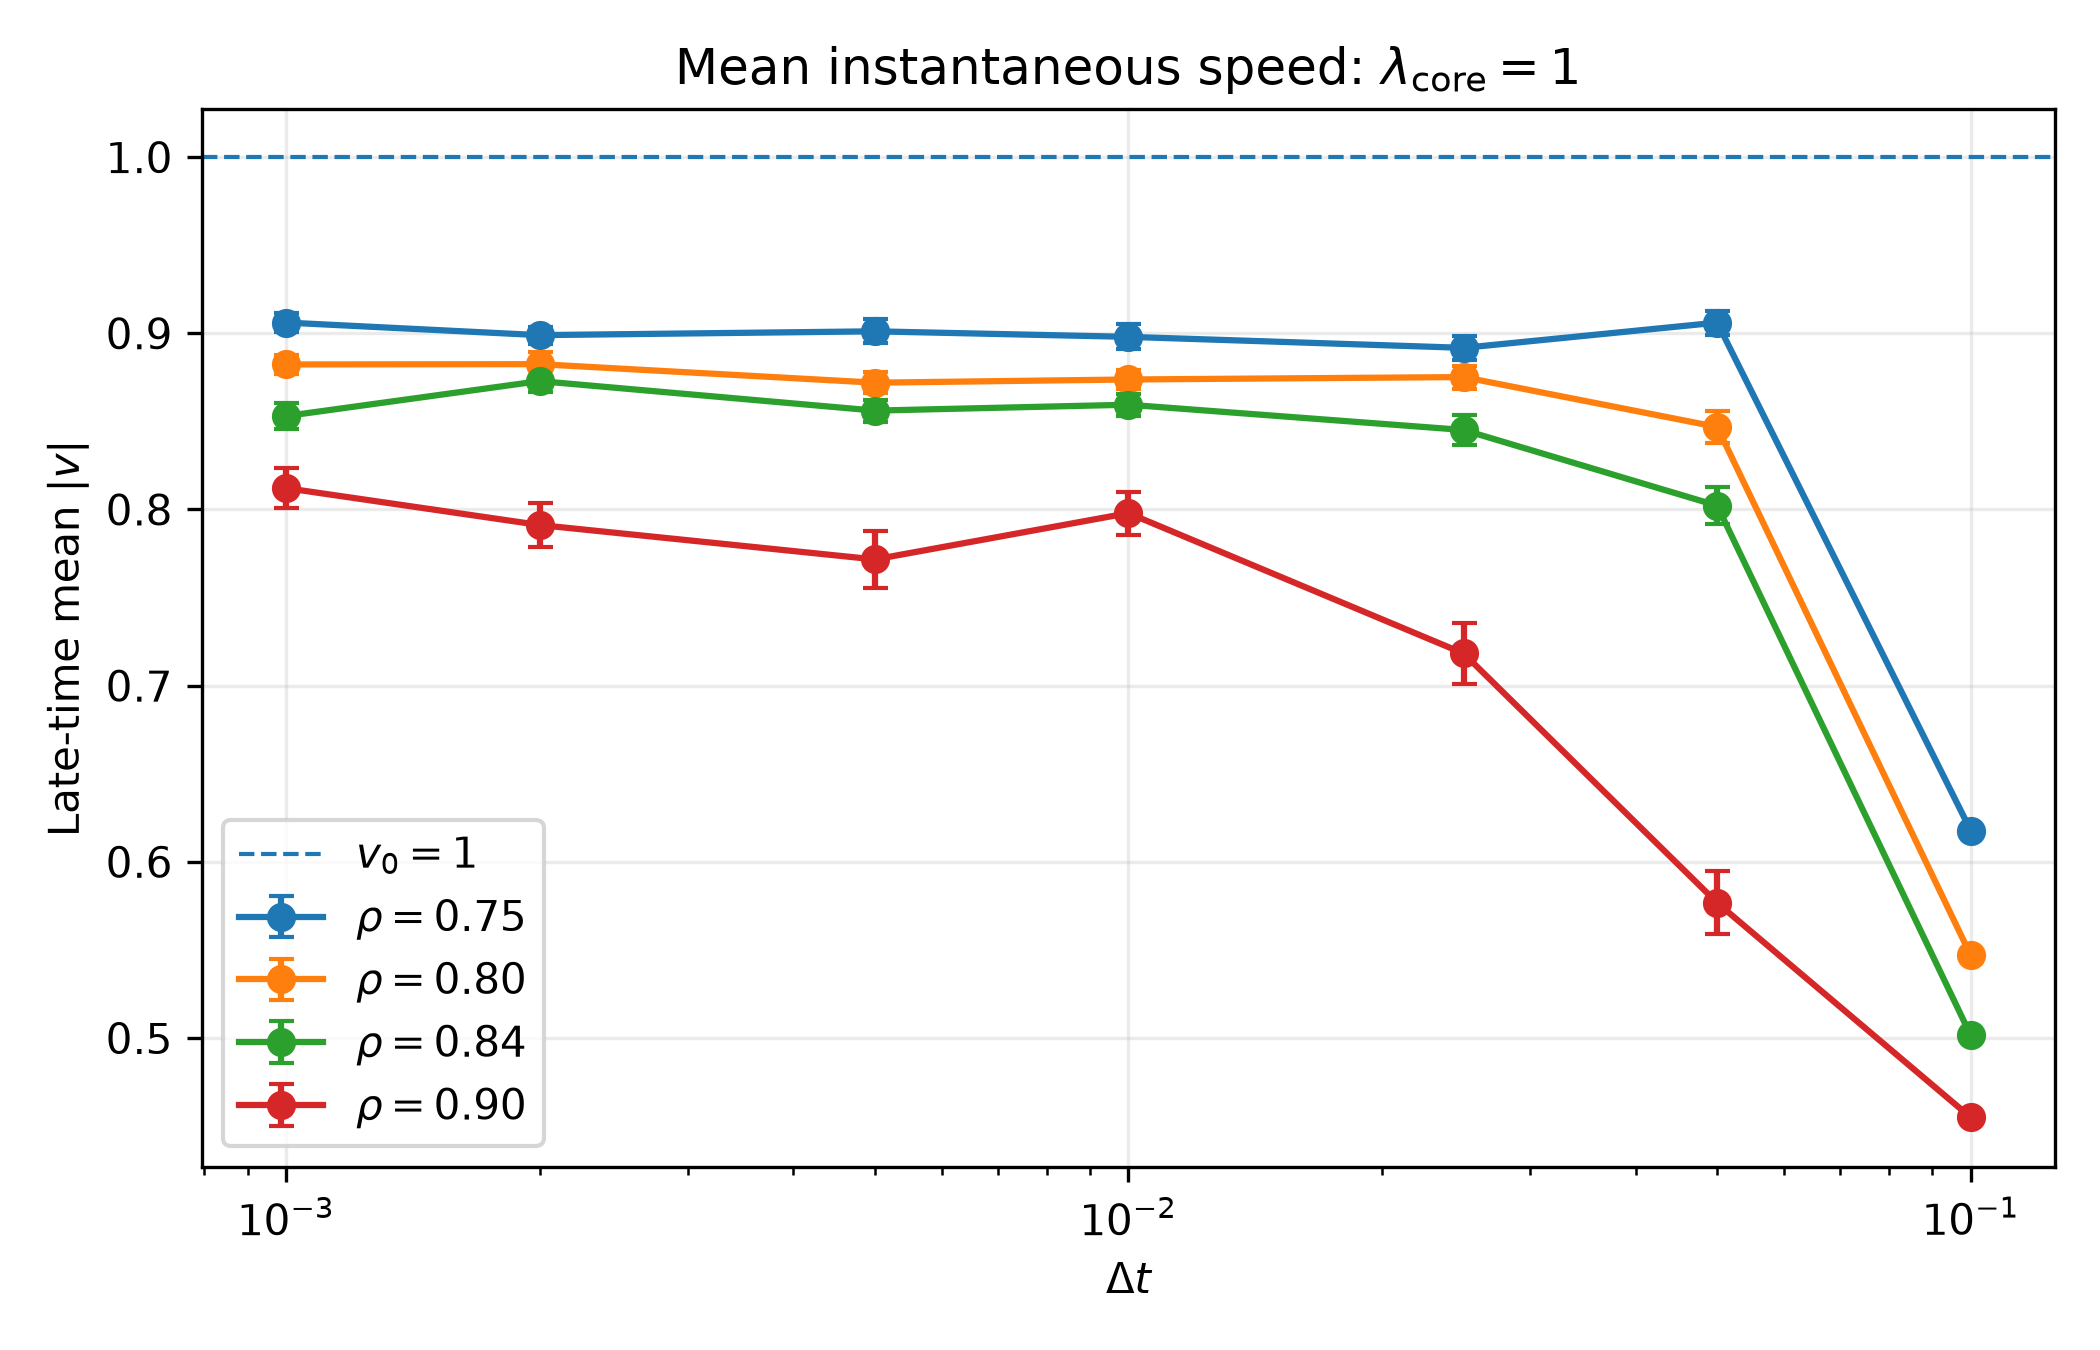
\includegraphics[width=\textwidth]
        {../figures/macro_ensemble_mean_speed_lambda_1.png}
        \caption{\(\lambda=1\).}
    \end{subfigure}
    \caption{
        Velocidad instantánea media en la ventana tardía. La línea de
        referencia \(v_0=1\) corresponde a la velocidad intrínseca de una
        célula completamente elongada y aislada.
    }
    \label{fig:mean_speed}
\end{figure}

\section{Elección de \texorpdfstring{\(\lambda\)}{lambda}}

El valor \(\lambda=0.1\) produce una dinámica numéricamente más suave y tolera
pasos temporales algo mayores. Sin embargo, esto ocurre a costa de permitir
superposiciones más profundas y de hacer intervenir con mucha mayor frecuencia
la regla de seguridad de contracción.

Por el contrario, \(\lambda=1\) cumple mejor el objetivo físico de la
regularización: mantiene las células fuera del núcleo de alta superposición y
reduce los rechazos de contracción a valores menores al \(1\%\), sin producir
velocidades mecánicas anómalas en el régimen convergido.

Por lo tanto, fijamos

\begin{equation}
\boxed{\lambda=1}.
\end{equation}

\section{Elección de \texorpdfstring{\(\Delta t\)}{Delta t}}

Para \(\lambda=1\), los distintos diagnósticos permiten distinguir tres
regímenes:

\begin{itemize}
    \item \(\Delta t\leq0.01\): régimen de pequeños pasos, con estadísticas
    macroscópicas, superposiciones y velocidades consistentes;
    \item \(\Delta t=0.025\): zona limítrofe, todavía numéricamente razonable
    pero con el comienzo de desviaciones sistemáticas;
    \item \(\Delta t\geq0.05\): aparecen cambios claros en el estado
    macroscópico y en las colas de superposición y velocidad.
\end{itemize}

Elegimos entonces el mayor paso que permanece claramente dentro del plateau,
sin trabajar en el borde del régimen estable:

\begin{equation}
\boxed{\Delta t=0.01}.
\end{equation}

Esta elección reduce el costo computacional en un factor diez respecto de
\(\Delta t=0.001\), utilizado como referencia, manteniendo un margen claro
respecto del inicio de las desviaciones.

\section{Conclusión}

La campaña permite fijar para las próximas simulaciones

\begin{equation}
\boxed{
\lambda=1,
\qquad
\Delta t=0.01
}.
\end{equation}

La elección de \(\lambda\) se basa principalmente en el mejor control físico
de las superposiciones, mientras que la elección de \(\Delta t\) se basa en la
estabilidad de las estadísticas de ensamble y de los diagnósticos
microscópicos.

Con estas dos elecciones cerradas, la siguiente validación del protocolo será
el número de orientaciones probadas en cada barrido de elongación,
\(n_{\mathrm{int}}\). Luego se estudiará el período entre barridos de
deformación \(T_{\mathrm{def}}\) y, finalmente, el umbral de seguridad de
contracción \(\xi_{\mathrm{safe}}\).

\end{document}
